\documentclass[a4paper,12pt,twoside]{memoir}

% Castellano
\usepackage[spanish,es-tabla]{babel}
\selectlanguage{spanish}
\usepackage[utf8]{inputenc}
\usepackage[T1]{fontenc}
\usepackage{lmodern} % scalable font
\usepackage{microtype}
\usepackage{placeins}

\RequirePackage{booktabs}
\RequirePackage[table]{xcolor}
\RequirePackage{xtab}
\RequirePackage{multirow}

% Links
\PassOptionsToPackage{hyphens}{url}\usepackage[colorlinks]{hyperref}
\hypersetup{
	allcolors = {red}
}

% Ecuaciones
\usepackage{amsmath}

% Rutas de fichero / paquete
\newcommand{\ruta}[1]{{\sffamily #1}}

% Párrafos
\nonzeroparskip

% Huérfanas y viudas
\widowpenalty100000
\clubpenalty100000

% Evitar solapes en el header
\nouppercaseheads

% Imagenes
\usepackage{graphicx}
\newcommand{\imagen}[2]{
	\begin{figure}[!h]
		\centering
		\includegraphics[width=0.9\textwidth]{#1}
		\caption{#2}\label{fig:#1}
	\end{figure}
	\FloatBarrier
}

\newcommand{\imagenflotante}[2]{
	\begin{figure}%[!h]
		\centering
		\includegraphics[width=0.9\textwidth]{#1}
		\caption{#2}\label{fig:#1}
	\end{figure}
}



% El comando \figura nos permite insertar figuras comodamente, y utilizando
% siempre el mismo formato. Los parametros son:
% 1 -> Porcentaje del ancho de página que ocupará la figura (de 0 a 1)
% 2 --> Fichero de la imagen
% 3 --> Texto a pie de imagen
% 4 --> Etiqueta (label) para referencias
% 5 --> Opciones que queramos pasarle al \includegraphics
% 6 --> Opciones de posicionamiento a pasarle a \begin{figure}
\newcommand{\figuraConPosicion}[6]{%
  \setlength{\anchoFloat}{#1\textwidth}%
  \addtolength{\anchoFloat}{-4\fboxsep}%
  \setlength{\anchoFigura}{\anchoFloat}%
  \begin{figure}[#6]
    \begin{center}%
      \Ovalbox{%
        \begin{minipage}{\anchoFloat}%
          \begin{center}%
            \includegraphics[width=\anchoFigura,#5]{#2}%
            \caption{#3}%
            \label{#4}%
          \end{center}%
        \end{minipage}
      }%
    \end{center}%
  \end{figure}%
}

%
% Comando para incluir imágenes en formato apaisado (sin marco).
\newcommand{\figuraApaisadaSinMarco}[5]{%
  \begin{figure}%
    \begin{center}%
    \includegraphics[angle=90,height=#1\textheight,#5]{#2}%
    \caption{#3}%
    \label{#4}%
    \end{center}%
  \end{figure}%
}
% Para las tablas
\newcommand{\otoprule}{\midrule [\heavyrulewidth]}
%
% Nuevo comando para tablas pequeñas (menos de una página).
\newcommand{\tablaSmall}[5]{%
 \begin{table}
  \begin{center}
   \rowcolors {2}{gray!35}{}
   \begin{tabular}{#2}
    \toprule
    #4
    \otoprule
    #5
    \bottomrule
   \end{tabular}
   \caption{#1}
   \label{tabla:#3}
  \end{center}
 \end{table}
}

%
%Para el float H de tablaSmallSinColores
\usepackage{float}

%
% Nuevo comando para tablas pequeñas (menos de una página).
\newcommand{\tablaSmallSinColores}[5]{%
 \begin{table}[H]
  \begin{center}
   \begin{tabular}{#2}
    \toprule
    #4
    \otoprule
    #5
    \bottomrule
   \end{tabular}
   \caption{#1}
   \label{tabla:#3}
  \end{center}
 \end{table}
}

\newcommand{\tablaApaisadaSmall}[5]{%
\begin{landscape}
  \begin{table}
   \begin{center}
    \rowcolors {2}{gray!35}{}
    \begin{tabular}{#2}
     \toprule
     #4
     \otoprule
     #5
     \bottomrule
    \end{tabular}
    \caption{#1}
    \label{tabla:#3}
   \end{center}
  \end{table}
\end{landscape}
}

%
% Nuevo comando para tablas grandes con cabecera y filas alternas coloreadas en gris.
\newcommand{\tabla}[6]{%
  \begin{center}
    \tablefirsthead{
      \toprule
      #5
      \otoprule
    }
    \tablehead{
      \multicolumn{#3}{l}{\small\sl continúa desde la página anterior}\\
      \toprule
      #5
      \otoprule
    }
    \tabletail{
      \hline
      \multicolumn{#3}{r}{\small\sl continúa en la página siguiente}\\
    }
    \tablelasttail{
      \hline
    }
    \bottomcaption{#1}
    \rowcolors {2}{gray!35}{}
    \begin{xtabular}{#2}
      #6
      \bottomrule
    \end{xtabular}
    \label{tabla:#4}
  \end{center}
}

%
% Nuevo comando para tablas grandes con cabecera.
\newcommand{\tablaSinColores}[6]{%
  \begin{center}
    \tablefirsthead{
      \toprule
      #5
      \otoprule
    }
    \tablehead{
      \multicolumn{#3}{l}{\small\sl continúa desde la página anterior}\\
      \toprule
      #5
      \otoprule
    }
    \tabletail{
      \hline
      \multicolumn{#3}{r}{\small\sl continúa en la página siguiente}\\
    }
    \tablelasttail{
      \hline
    }
    \bottomcaption{#1}
    \begin{xtabular}{#2}
      #6
      \bottomrule
    \end{xtabular}
    \label{tabla:#4}
  \end{center}
}

%
% Nuevo comando para tablas grandes sin cabecera.
\newcommand{\tablaSinCabecera}[5]{%
  \begin{center}
    \tablefirsthead{
      \toprule
    }
    \tablehead{
      \multicolumn{#3}{l}{\small\sl continúa desde la página anterior}\\
      \hline
    }
    \tabletail{
      \hline
      \multicolumn{#3}{r}{\small\sl continúa en la página siguiente}\\
    }
    \tablelasttail{
      \hline
    }
    \bottomcaption{#1}
  \begin{xtabular}{#2}
    #5
   \bottomrule
  \end{xtabular}
  \label{tabla:#4}
  \end{center}
}



\definecolor{cgoLight}{HTML}{EEEEEE}
\definecolor{cgoExtralight}{HTML}{FFFFFF}

%
% Nuevo comando para tablas grandes sin cabecera.
\newcommand{\tablaSinCabeceraConBandas}[5]{%
  \begin{center}
    \tablefirsthead{
      \toprule
    }
    \tablehead{
      \multicolumn{#3}{l}{\small\sl continúa desde la página anterior}\\
      \hline
    }
    \tabletail{
      \hline
      \multicolumn{#3}{r}{\small\sl continúa en la página siguiente}\\
    }
    \tablelasttail{
      \hline
    }
    \bottomcaption{#1}
    \rowcolors[]{1}{cgoExtralight}{cgoLight}

  \begin{xtabular}{#2}
    #5
   \bottomrule
  \end{xtabular}
  \label{tabla:#4}
  \end{center}
}




\graphicspath{ {./img/} }

% Capítulos
\chapterstyle{bianchi}
\newcommand{\capitulo}[2]{
	\setcounter{chapter}{#1}
	\setcounter{section}{0}
	\setcounter{figure}{0}
	\setcounter{table}{0}
	\chapter*{#2}
	\addcontentsline{toc}{chapter}{#2}
	\markboth{#2}{#2}
}

% Apéndices
\renewcommand{\appendixname}{Apéndice}
\renewcommand*\cftappendixname{\appendixname}

\newcommand{\apendice}[1]{
	%\renewcommand{\thechapter}{A}
	\chapter{#1}
}

\renewcommand*\cftappendixname{\appendixname\ }

% Formato de portada
\makeatletter
\usepackage{xcolor}
\newcommand{\tutor}[1]{\def\@tutor{#1}}
\newcommand{\course}[1]{\def\@course{#1}}
\definecolor{cpardoBox}{HTML}{E6E6FF}
\def\maketitle{
  \null
  \thispagestyle{empty}
  % Cabecera ----------------
\noindent\includegraphics[width=\textwidth]{cabecera}\vspace{1cm}%
  \vfill
  % Título proyecto y escudo informática ----------------
  \colorbox{cpardoBox}{%
    \begin{minipage}{.8\textwidth}
      \vspace{.5cm}\Large
      \begin{center}
      \textbf{TFG del Grado en Ingeniería Informática}\vspace{.6cm}\\
      \textbf{\LARGE\@title{}}
      \end{center}
      \vspace{.2cm}
    \end{minipage}

  }%
  \hfill\begin{minipage}{.20\textwidth}
    \includegraphics[width=\textwidth]{escudoInfor}
  \end{minipage}
  \vfill
  % Datos de alumno, curso y tutores ------------------
  \begin{center}%
  {%
    \noindent\LARGE
    Presentado por \@author{}\\ 
    en Universidad de Burgos --- \@date{}\\
    Tutor: \@tutor{}\\
  }%
  \end{center}%
  \null
  \cleardoublepage
  }
\makeatother


% Datos de portada
\title{Vulnerabilidad de redes de paquetes software II\\Documentación Técnica}
\author{Daniel Alonso Báscones}
\tutor{Carlos López Nozal}
\date{\today}

\begin{document}

\maketitle



\cleardoublepage



%%%%%%%%%%%%%%%%%%%%%%%%%%%%%%%%%%%%%%%%%%%%%%%%%%%%%%%%%%%%%%%%%%%%%%%%%%%%%%%%%%%%%%%%



\frontmatter


\clearpage

% Indices
\tableofcontents

\clearpage

\listoffigures

\clearpage

\listoftables

\clearpage

\mainmatter

\appendix

\apendice{Plan de Proyecto Software}

\section{Introducción}

El proyecto propuesto se centra en el desarrollo de la herramienta \textit{OLIVIA-Finder}, 
la cual ha sido diseñada con el objetivo de extraer datos de paquetes y sus dependencias de 
los repositorios de software \textit{CRAN, Bioconductor, PyPI y npm}. 

Dado que la herramienta en sí misma carece de elementos visuales o atractivos más allá 
de la presentación de los datos en forma de una lista de enlaces entre nodos de la red, 
se ha decidido complementarla con un análisis básico de las redes generadas desde la perspectiva 
de la ciencia de redes. Esto se realiza con el propósito de evitar que el trabajo resulte monótono 
y brindar un enfoque más completo y enriquecedor al proyecto.

En general, el proyecto se puede describir en tres etapas fundamentales. 
La primera etapa consiste en una exhaustiva investigación y documentación, donde se realiza un estudio 
en profundidad de los repositorios \textit{CRAN, Bioconductor, PyPI y npm}, así como de las técnicas y herramientas 
utilizadas para la extracción de datos y análisis de redes de dependencias. Esta etapa sienta las bases teóricas 
necesarias para comprender el contexto en el que se desarrollará la herramienta y el análisis posterior.

La segunda etapa se enfoca en el diseño y desarrollo de la herramienta \textit{OLIVIA-Finder}. 
Aquí, se aplican los conocimientos adquiridos durante la etapa de investigación para implementar una solución 
eficiente y robusta que permita la extracción de datos de los repositorios mencionados. 
Se deben tener en cuenta diversos aspectos técnicos, como el manejo de solicitudes web, el procesamiento de datos 
y la manipulación de estructuras de red.

La tercera etapa del proyecto implica el análisis experimental de las redes generadas. 
Una vez obtenidos los datos de los paquetes y sus dependencias, se aplican técnicas de la ciencia de redes 
para examinar características importantes, como la \textit{centralidad de grado}, el algoritmo \textit{PageRank} y 
otras métricas relevantes. Este análisis proporciona una comprensión más profunda de la estructura 
y las propiedades de las redes de dependencias en los repositorios estudiados, permitiendo identificar 
paquetes críticos, vulnerabilidades potenciales y relaciones significativas entre los elementos de la red.

\section{Planificación temporal}

En el ámbito de los proyectos modernos de software, es común utilizar metodologías ágiles, como \textit{Scrum} 
o \textit{Kanban}. Estas metodologías reconocen la naturaleza dinámica del proceso iterativo que implica el 
establecimiento de requisitos, diseño, desarrollo y validación de un producto de software. Por lo tanto, 
se enfocan en la planificación adaptativa y la mejora continua a través de entregas tempranas.

Sin embargo, en nuestro caso, debemos cuestionar la aplicabilidad práctica de las metodologías ágiles 
tal como están concebidas. Esto se debe a que el conjunto de partes interesadas, que se limita a un 
cliente académico prototípico, y sobre todo al hecho de que el equipo de trabajo es unipersonal. Estas 
circunstancias particulares plantean dudas sobre la eficacia de la implementación de las metodologías 
ágiles en nuestro contexto.

No obstante, podemos establecer similitudes entre nuestro proceso y el marco de trabajo \textit{Scrum}, 
debido a la presencia de \textit{sprints}. Aunque no hemos seguido rigurosamente la estructura de los \textit{sprints} 
debido a la falta de objetivos claramente definidos en el proyecto, los \textit{sprints} nos han permitido 
representar la actividad realizada y las etapas en las que hemos dividido el trabajo.

Por otro lado, se ha de tener en cuenta que las tareas de investigación incluidas en el proyecto son 
difíciles de planificar. El proceso de investigación implica continuos replanteamientos y el alcance de 
los resultados debe ser constantemente modelado o redefinido a medida que avanzamos dentro del límite 
temporal del que se dispone.

\subsection{Sprint 0: Kick of meeting}

Este \textit{sprint} representó nuestra primera aproximación a la temática del proyecto. Desde el principio, quedó 
claro que el modelo matemático proporcionado por OLIVIA en el Trabajo de Fin de Grado anterior estaba más allá de 
nuestra comprensión absoluta, y nuestro enfoque se centraría principalmente en la experimentación.

Por lo tanto, fue necesario realizar un esfuerzo inicial para comprender los fundamentos básicos de lo que el modelo 
de \textit{OLIVIA} nos permitía hacer. En este sentido, los Jupyter Notebooks proporcionados en el TFG anterior fueron de 
gran utilidad, ya que mostraban la funcionalidad en casos de estudio concretos y ofrecían un análisis complementario.

Desde el principio, nos encontramos con problemas técnicos. En primer lugar, las dependencias de \textit{OLIVIA} requieren una 
actualización, ya que se están utilizando versiones algo desactualizadas de algunos paquetes y herramientas de análisis, 
y el \textit{Dependabot de GitHub} insiste en su actualización \textit{``Bump numpy from 1.18.5 to 1.22.0''}. En concreto, 
se ha identificado que esta versión de \textit{NumPy} presenta vulnerabilidades de alto riesgo, como la referida al 
\textit{NumPy NULL Pointer Dereference}.

Sin embargo, no es posible actualizar la biblioteca, ya que existen métodos esenciales para la funcionalidad 
implementada en \textit{OLIVIA} que se han vuelto obsoletos en la versión actualizada. Además, en cuanto a la versión de Python, 
el código debe ejecutarse en la versión 3.8 debido a la presencia de dependencias clave para OLIVIA, como \textit{intbitset}, 
que no están disponibles para otras versiones de Python. Esto supuso un problema al ejecutar los notebooks 
en \textit{Google Colab} debido a las dificultades para instalar la versión específica de Python que requeríamos.

Además, fue necesario realizar una introducción a la temática mediante una lectura superficial de la memoria del 
TFG de OLIVIA. Esto también nos permitió familiarizarnos con el hecho de que estas memorias se redactan 
utilizando \LaTeX, una tecnología que nos resultaba completamente desconocida en ese momento.

En conclusión, este \textit{sprint} inicial implicó la familiarización con el modelo de OLIVIA, la comprensión de 
sus fundamentos y la resolución de desafíos técnicos relacionados con las dependencias y las versiones de Python. 
Además, se llevó a cabo una introducción a la temática a través del estudio de la memoria del TFG anterior, lo que 
también nos permitió adquirir conocimientos sobre el uso de \LaTeX en la redacción de documentos científicos.

La duración de este \textit{sprint} ha sido de 30 días aproximadamente, realizando 2 reuniones y 
con unas 25 horas de trabajo.

\subsection{Sprint 1 - Data collection}

En esta etapa de investigación nos enfocamos en el manejo de datos. Inicialmente, utilizamos el conjunto de datos 
de \textit{libraries.io}, el cual resultó útil desde una perspectiva histórica. Sin embargo, presentó importantes 
limitaciones, como la falta de actualización periódica. Al enfrentarnos a los desafíos derivados de este conjunto 
de datos, pudimos constatar que trabajar con grandes volúmenes de datos no es trivial. Fue necesario utilizar un 
disco duro externo para almacenar el conjunto de datos, del cual solo nos interesaba la lista de enlaces entre 
paquetes y dependencias contenida en uno de los archivos CSV. Debido a la gran cantidad de líneas y su considerable 
tamaño, resultó difícil manipular y filtrar los datos.

La falta de actualización de los datos fue un aspecto clave a mejorar, por lo cual exploramos otras fuentes de información, 
como la API de \textit{libraries.io} y el conjunto de datos de \textit{BigQuery} proporcionado por los mismos desarrolladores. 
El uso de la API quedó descartado debido a sus limitaciones técnicas para realizar un escaneo completo del repositorio. 
Por otro lado, el conjunto de datos de \textit{BigQuery} también presentó problemas similares a los archivos CSV en 
términos de falta de actualización.

Como alternativa, se propuso utilizar técnicas de \textit{web scraping} para recolectar información de los sitios web 
de los repositorios de software de nuestro interés, comenzando con la recolección de información de CRAN. Este esfuerzo 
dio resultados positivos, y logramos obtener una lista actualizada de la red de CRAN. Los éxitos obtenidos en este 
proceso nos llevaron a considerar el desarrollo de una herramienta que pudiera obtener esta información para los 
repositorios de interés, ya que esto generaría un nuevo conjunto de datos utilizable en OLIVIA y en trabajos anteriores 
que hayan utilizado datos de \textit{libraries.io}, lo que permitiría actualizar sus resultados de manera significativa.

Como resultado al finalizar este \textit{sprint}, logramos obtener una red actualizada de CRAN gracias a que desarrollamos 
un prototipo básico pero todavía inmaduro de un código en Python que nos permitió realizar la recolección de datos.

Es importante destacar que durante este \textit{sprint} se abordó uno de los principales desafíos que hemos enfrentado. 
Como era de esperar, los servidores web implementan medidas de seguridad para evitar comportamientos maliciosos. Debido 
a la naturaleza del proceso de escaneo de un repositorio, que implica realizar numerosas solicitudes web a un mismo servidor 
desde una misma dirección IP en un período de tiempo relativamente corto, esta actividad a menudo resulta en la prohibición temporal de acceso al servidor web para los equipos asociados a esa dirección IP. Para solucionar este problema, se implementó la funcionalidad de ocultar las solicitudes detrás de servidores proxy, que enmascaran la dirección IP de origen al servidor web. Por lo tanto, fue necesario desarrollar esta funcionalidad para que fuera posible llevar a cabo esta tarea.

En conclusión, este \textit{sprint} fue clave para obtener un conjunto de datos actualizado y establecer los primeros 
pasos en el desarrollo de una herramienta de recolección de datos. Además, se logró resolver el desafío de la prohibición 
de acceso a los serv

idores web mediante la implementación de rotación de proxy. Estos avances sientan las bases para continuar con el desarrollo 
del proyecto y alcanzar los objetivos planteados.

La duración de este \textit{sprint} ha sido aproximadamente de 30 días, que en nuestra metodología de trabajo equivalen 
aproximadamente a 2 reuniones y a 60 horas de trabajo.

\subsection{Sprint 2 - Library implementation and interpretation of some data}

En esta etapa, nuestro enfoque se centró en el desarrollo de una herramienta genérica con el propósito de llevar a cabo 
una extracción sencilla de la red de dependencias de los repositorios \textit{CRAN}, \textit{Bioconductor}, \textit{PyPI} 
y \textit{npm}. Nos enfrentamos al primer desafío de obtener una lista completa de los paquetes disponibles en cada 
repositorio, que serviría como punto de partida para nuestra recopilación de datos. Cabe destacar que esta tarea no 
esulta sencilla en la mayoría de los casos, ya que dichas listas no siempre están disponibles.

Es importante mencionar que cada repositorio de software presenta sus peculiaridades distintivas. En el caso particular 
de \textit{CRAN} y \textit{Bioconductor}, el proceso se basó exclusivamente en técnicas de \textit{web scraping}, 
aprovechando los datos de interés que se encuentran directamente en las listas de paquetes publicadas en sus respectivos 
sitios web.

El análisis de \textit{CRAN} resultó ser el más sencillo de todos, ya que su página web es simple, robusta y aparentemente 
sólida a lo largo del tiempo, lo que proporciona una implementación bastante estable para este repositorio. Por otro 
lado, inicialmente se esperaba que \textit{Bioconductor} fuese más sencillo debido a la menor cantidad de paquetes en 
comparación con los otros repositorios en los que estamos trabajando. Sin embargo, nos encontramos con un problema en 
el servidor web de \textit{Bioconductor}, específicamente en la página que muestra el listado de paquetes disponibles, 
ya que no era accesible mediante una simple solicitud web, como las que solemos realizar utilizando la biblioteca 
\textit{requests} de Python.

En \textit{Bioconductor}, se utilizaba JavaScript para cargar dinámicamente la lista de paquetes en tiempo de ejecución 
sobre la página. Esta situación dificulta la obtención de los datos, ya que la biblioteca \textit{requests} no es 
compatible con la carga de JavaScript. Como alternativa, tuvimos que recurrir a la biblioteca \textit{selenium}, la 
cual ofrece funcionalidades más avanzadas al actuar como un navegador \textit{headless} (sin interfaz gráfica) que 
se comporta de manera similar a un navegador de escritorio convencional al que estamos acostumbrados, pero que admite 
la automatización de tareas. Gracias a \textit{selenium}, logramos extraer la lista de paquetes de \textit{Bioconductor} 
y, a partir de ella, procedimos de manera similar a como lo habíamos hecho anteriormente, obteniendo los datos de interés 
mediante técnicas de \textit{web scraping}.

El repositorio \textit{PyPI}, también publica una lista de paquetes. Sin embargo, es importante destacar que esta 
lista contiene muchos paquetes obsoletos e inexistentes, lo que la convierte en un punto de partida necesario pero 
no del todo óptimo. Utilizando esta lista de paquetes y aprovechando la API proporcionada por \textit{PyPI} para 
obtener metadatos de los paquetes, pudimos extraer la red de dependencias correspondiente.

En esta etapa, nos percatamos del tiempo considerablemente elevado requerido para llevar a cabo esta recopilación, 
así como de la necesidad de cuidar la implementación de la herramienta para evitar el desperdicio de memoria. 
Estos problemas surgidos debido al tamaño de los datos nos proporcionan una perspectiva clara de la importancia de 
gestionar eficientemente los recursos cuando se trabaja con cantidades masivas de información. En cuanto al tiempo 
necesario para la recolección, se realizó un esfuerzo por optimizar el proceso mediante técnicas de concurrencia, 
lo cual nos permitió realizar solicitudes web de forma concurrente en lugar de secuencial, como habíamos estado haciendo 
hasta ese momento. Estas mejoras significativas en el rendimiento de la herramienta se tradujeron en una reducción 
significativa del tiempo requerido y el consumo de memoria.

Finalmente, logramos generar el conjunto de datos para el repositorio \textit{npm}. Es importante destacar que este 
repositorio ha sido el más desafiante de abordar. En primer lugar, no existe una forma sencilla de obtener una lista 
completa de los paquetes existentes en \textit{npm}. Además, el repositorio oficial de paquetes no es único, ya que 
existen repositorios espejo (\textit{mirrors}) alternativos que difieren tanto en el número de paquetes como en los 
paquetes que contienen. Para abordar este problema, decidimos utilizar la lista de paquetes que pudimos extraer de 
uno de estos \textit{mirrors} y complementar con los paquetes que teníamos en el conjunto de datos de \textit{libraries.io}. 
De esta manera, obtuvimos una lista de nombres de paquetes a los cuales dirigir nuestros esfuerzos. A partir de esta 
lista, aplicamos la metodología utilizada previamente para el resto de los repositorios. En el caso de \textit{npm}, 
gracias a su API, pudimos recopilar los metadatos necesarios para construir el conjunto de datos correspondiente.

Llevar a cabo este \textit{sprint} ha supuesto una duración de 60 días, lo que aproximadamente corresponde con unas 
3 reuniones y alrededor de 150 horas de trabajo.

\subsection{Sprint 3 - Library refactoring}

Tras el análisis de los datos recolectados, observamos que los conjuntos de datos de \textit{libraries.io} proporcionan 
información sobre todas las versiones existentes de un paquete. En otras palabras, consideramos como \textit{dependencias} 
de un paquete todas las dependencias que hayan existido para cada una de sus versiones. Sin embargo, desde una perspectiva 
de desarrollo de software, esto no es correcto, ya que sobrecargamos las dependencias de un paquete con dependencias de 
versiones antiguas que ya no se utilizan en el ciclo de vida actual de esas bibliotecas. Por lo tanto, es importante tener 
en cuenta esta información en los análisis posteriores que realicemos, donde será necesario aplicar un filtrado adecuado 
si deseamos utilizar los datos de \textit{libraries.io}.
Otro aspecto interesante es que no todas las \textit{dependencias} de un paquete se encuentran presentes en el repositorio 
al que pertenece ese paquete, e incluso es posible que no utilicen el mismo lenguaje de programación. Tomemos como ejemplo 
un paquete en Python que depende de un binario escrito en C. Este fenómeno es muy común en la red de \textit{Bioconductor}, 
cuyos paquetes dependen en gran medida de paquetes existentes en \textit{CRAN}. 
A estas dependencias las hemos bautizado como \textit{dependencias foráneas}.

Con el objetivo de mejorar la funcionalidad y flexibilidad de la biblioteca, se llevó a cabo una refactorización del 
diseño para adaptarlo y permitir el uso y la combinación de diversas fuentes de datos. Se proporciona soporte para 
\textit{web scraping}, conjuntos de datos en formato \textit{CSV}, la API de \textit{libraries.io} y repositorios de 
\textit{GitHub}.
El uso combinado de diferentes fuentes de datos nos brinda la capacidad de buscar en fuentes alternativas cuando un 
paquete solicitado no se encuentra en la fuente principal. El soporte de archivos \textit{CSV} nos permite considerar 
los conjuntos de datos de \textit{libraries.io} como fuente de información, tanto a través de su API como de los archivos 
en sí. La implementación para repositorios de \textit{GitHub} nos proporciona información adicional al utilizar 
\textit{GitHub} como fuente de datos, ya que es el sistema de control de versiones por excelencia donde se encuentran 
la mayoría de los proyectos de software de código abierto publicados. De esta manera, tenemos acceso a un repositorio 
de un nivel inferior, ya que no pertenece a un gestor de paquetes específico de un lenguaje de programación, sino que 
se basa su relevancia principalmente en un ámbito más cercano al desarrollo.
Además, la biblioteca ofrece otras funcionalidades, como la obtención en tiempo de ejecución de una red de dependencias 
transitiva para un paquete en particular. También proporciona persistencia de datos en forma de objetos serializados y 
la capacidad de exportar datos en formato \textit{CSV} compatible con \textit{OLIVIA}.

Una vez concluida esta etapa, procedimos a publicar los conjuntos de datos en \textit{Zenodo}, con el fin de hacerlos 
accesibles para la comunidad científica. Además, dedicamos nuestros esfuerzos a mejorar la documentación del código 
fuente y generar una documentación completa de la biblioteca. Esta documentación está diseñada para ser accesible desde
 la web y se encuentra alojada en \textit{GitHub Pages}.
La publicación de los conjuntos de datos en \textit{Zenodo} permite a otros investigadores y desarrolladores acceder a 
los datos recopilados y utilizarlos en sus propios proyectos o investigaciones. De esta manera, promovemos la transparencia 
y el intercambio de información entre la comunidad científica.
En cuanto a la documentación de la biblioteca, nos esforzamos por ofrecer una guía clara y concisa sobre cómo utilizar 
la biblioteca, qué funcionalidades y características ofrece, así como ejemplos de uso. La documentación se ha estructurado 
de manera que sea fácil de navegar y buscar información relevante. Al alojarla en \textit{GitHub Pages}, proporcionamos 
un acceso práctico y amigable para los usuarios, quienes pueden acceder a la documentación directamente desde el sitio web
 del proyecto en \textit{GitHub}.
Este \textit{sprint} ha sido difícil de calcular el tiempo que ha llevado realizarlo, debido a que ha habido saltos 
hacia \textit{sprints} anteriores cuando estamos trabajando en este. Ha sido uno de los más complejos. Se calcula un 
periodo de 60 días, 4 reuniones y aproximadamente 150 horas de trabajo.

\subsection{Sprint 4 - Análisis de datos}

En la etapa final de este estudio, se utilizaron los datos recopilados para realizar un análisis con una perspectiva 
evolutiva de las redes de dependencias presentes en los repositorios \textit{CRAN}, \textit{Bioconductor}, \textit{PyPI} 
y \textit{npm}, utilizando la ciencia de redes como marco de referencia.

En este análisis, se lleva a cabo una comparativa entre el estado de la red según los datos obtenidos de \textit{libraries.io} 
y los datos obtenidos mediante \textit{web scraping}. Se realiza un análisis desde el punto de vista de la centralidad de 
grado y el algoritmo \textit{PageRank}, con el objetivo de identificar y argumentar cuáles son los paquetes más vulnerables 
y por qué. Además, se calculan algunas de las métricas proporcionadas por el modelo de red de \textit{OLIVIA} y se establecen 
relaciones entre ellas.

Este análisis ofrece una perspectiva a nivel micro al examinar los extremos de la red, como los paquetes más destacados, y 
una visión más macro al analizar distribuciones y propiedades más generales, como el grado medio. Su objetivo principal es 
proporcionar una comprensión más profunda de la composición de estas redes de dependencias, sin abordar un análisis exhaustivo 
de toda la red.

Este \textit{sprint} en cuanto a duración fue el más corto y de una duración de 15 días, en los que hubo 3 reuniones, y 
aproximadamente ocupó unas 30 horas de trabajo.


\section{Estudio de viabilidad}

Considerando la dirección y metas de las actividades planificadas, procederemos a evaluar la factibilidad de las mismas, 
teniendo en cuenta su enfoque como un proyecto de investigación, desarrollo e innovación.

\subsection{Viabilidad económica}

\subsubsection{Presupuesto}

Para realizar una estimación precisa del presupuesto del proyecto, hemos considerado diferentes aspectos relacionados 
con los costos involucrados. En primer lugar, hemos establecido una tarifa base de \textit{15€} por hora de trabajo 
para el autor del proyecto, incluyendo los costos salariales, complementos y seguridad social. Cabe destacar que no 
se han identificado gastos significativos en material o hardware, a excepción del consumo eléctrico durante la recolección 
de datos.

En cuanto al software utilizado, nos complace informar que todos los productos empleados en el desarrollo del proyecto 
han sido de coste cero. Sin embargo, es importante mencionar que existe la posibilidad de incurrir en gastos adicionales 
si se decide utilizar servicios de computación en la nube de pago, aunque estos no son estrictamente necesarios para el
 proyecto.

En términos de \textit{costos indirectos}, los cuales abarcan los gastos generales imputables al proyecto, los hemos 
incluido en la partida correspondiente. Siguiendo una práctica común, hemos asignado un \textit{15\%} del presupuesto 
de personal directo como gastos indirectos. De esta manera, hemos obtenido una aproximación al presupuesto total del 
proyecto de $415 \text{ horas} \times 15\textit{€}/\text{hora} \times 1.15 = 7158.75\textit{€}$. Es importante señalar que esta cifra 
no contempla posibles gastos derivados de la publicación y difusión de los resultados, los cuales podrían añadirse en 
etapas posteriores.

En cuanto al salario del profesor, quien cuenta con una mayor experiencia y conocimientos especializados, se ha 
establecido una tarifa base de \textit{30€} por hora. Considerando que ha habido un total de 14 reuniones, cada 
una con una duración aproximada de \textit{1.5} horas, y aplicando los mismos gastos indirectos del \textit{15\%}, 
el costo total asociado a estas reuniones sería de $14 \text{ reuniones} \times 1.5  \text{ horas} \times 30\textit{€}/\text{hora} \times 1.15 = 724\textit{€}$.

En resumen, según nuestras estimaciones, el desarrollo de este proyecto conllevaría un costo aproximado de \textit{9283.5€}. 
Este presupuesto abarca los salarios del autor del trabajo y del profesor, los gastos indirectos correspondientes y otros 
aspectos operativos relevantes.

Por último, es importante mencionar que, debido a la naturaleza del proyecto como una iniciativa de código abierto e 
investigación, no se permite la venta ni la comercialización del producto resultante con fines comerciales. El objetivo 
principal es promover la colaboración y el intercambio de conocimientos en la comunidad científica.

\subsubsection{Financiación}

Los programas nacionales o europeos de financiación destinados a la \textit{investigación, desarrollo e innovación (I+D+i)} 
podrían constituir una opción viable para sufragar total o parcialmente el proyecto. Por lo general, resulta necesario contar 
con una \textit{afiliación} a un marco empresarial o académico específico que permita acceder a los 
diversos \textit{instrumentos de financiación} disponibles.

Una interesante posibilidad que merece ser estudiada, y que ha cobrado relevancia en el contexto del movimiento 
de \textit{Ciencia Abierta}, es el \textit{crowdfunding}. Esta modalidad persigue la obtención de dinero  
para el proyecto mediante contribuciones económicas realizadas por personas interesadas en contribuir al progreso 
de la \textit{investigación científica transparente} y con \textit{resultados públicos, accesibles y gratuitos}. Algunos ejemplos son
\textit{Kickstarter} o \textit{Indiegogo}.

En el ámbito del \textit{crowdfunding}, es de una \textit{importancia capital} presentar de forma atractiva 
la idea del proyecto, destacando su \textit{relevancia e impacto} en la \textit{comunidad científica} y en 
la sociedad en general. Asimismo, es fundamental establecer una estrategia de comunicación efectiva 
para alcanzar a potenciales colaboradores y motivarlos a realizar sus aportaciones económicas.


\subsection{Viabilidad legal}

La viabilidad legal del proyecto software que hemos desarrollado es favorable, considerando las siguientes características:

\textbf{Naturaleza \textit{opensource} y gratuita:} 

Todo el proyecto ha sido diseñado bajo una filosofía de código abierto y gratuito, 
lo que implica que el software y sus componentes están disponibles para ser utilizados, modificados y distribuidos sin 
restricciones. Esta elección nos permite fomentar la colaboración y el acceso abierto a la tecnología desarrollada.

La biblioteca que hemos desarrollado para el proyecto tiene 
una naturaleza experimental y no comercial. Esto implica que su propósito es explorar nuevas ideas y soluciones tecnológicas, 
sin intención de generar beneficios económicos directos a través de su venta o licenciamiento.

\textbf{Recursos extraídos de la red:}

Los recursos utilizados en el proyecto, como bibliotecas y herramientas, han sido obtenidos 
de fuentes abiertas y accesibles en Internet. Al utilizar estos recursos, hemos respetado las condiciones y términos de 
uso establecidos por los autores y las licencias correspondientes.

El conjunto de datos utilizado en el proyecto ha sido recolectado de fuentes 
accesibles en la red, donde cualquier persona puede acceder a ellos. Nos hemos esforzado en recopilar y proporcionar estos 
datos a la comunidad, siguiendo los principios de transparencia y acceso abierto. En el caso de uso de estos datos, solo 
exigimos la atribución a los autores del Trabajo Fin de Grado correspondiente.

Aprovechamos este momento para dar atribucion al creador del conjunto de datos de \textit{libraries.io} llamado \textit{Tidelift}.

\textbf{Licencia de código abierto:}

Con respecto a la clasificación de la licencia adecuada para el proyecto, considerando los aspectos mencionados, una opción 
apropiada podría ser la licencia \textit{Creative Commons Attribution-ShareAlike 4.0 International (CC BY-SA 4.0)}. Esta licencia 
permite utilizar, modificar y distribuir el software y sus componentes, siempre y cuando se atribuya adecuadamente a los 
autores originales y se comparta bajo una licencia similar. Esta elección refuerza los principios de acceso abierto y 
fomenta la colaboración en la comunidad de desarrolladores y usuarios del software.



\apendice{Especificación de Requisitos}

\section{Introducción}
La herramienta \textit{Olivia Finder} tiene como objetivo principal proporcionar
una gestión eficiente de paquetes y dependencias de diferentes repositorios, como
\textit{PyPI}, \textit{npm}, \textit{CRAN} y \textit{Bioconductor}. Para lograr esto,
hemos identificado una serie de requisitos funcionales que guiarán el diseño y la
implementación del sistema.

El primer requisito funcional, \texttt{RF-1}, se centra en el almacenamiento eficiente
y el acceso rápido a la información de paquetes y dependencias. Es fundamental que el
sistema pueda almacenar esta información de manera eficiente para evitar demoras
significativas en la recuperación de datos. Además, el acceso rápido a la información
permitirá un rendimiento óptimo del sistema.

La extensibilidad y flexibilidad de la estructura de datos es abordada por el
requisito \texttt{RF-2}. Dado que los repositorios y las relaciones de dependencia
pueden evolucionar con el tiempo, es esencial que la estructura de datos utilizada sea
adaptable y pueda ser modificada o ampliada sin dificultades. Esto garantizará que el
sistema pueda adaptarse a futuras modificaciones en los repositorios y en las necesidades
de gestión de dependencias.

El requisito \texttt{RF-3} se enfoca en la representación específica de paquetes mediante
una estructura de datos adecuada. Cada paquete debe tener una representación clara y
precisa, que incluya los atributos relevantes para dicho paquete. Esto facilitará la
gestión y el análisis de los paquetes y sus dependencias dentro del sistema.

El requisito \texttt{RF-4} se refiere a la representación y exportación genérica de la
red de dependencias en diferentes formatos. Es importante que la red de dependencias
pueda ser representada en formatos genéricos de grafo dirigido, así como en otros formatos
como diccionarios, listas o dataframes. Esta versatilidad en la representación y exportación
permitirá un uso más amplio de la red de dependencias en diferentes herramientas y análisis.

La reconstrucción de las estructuras de datos a través de la persistencia es abordada por
el requisito \texttt{RF-5}. El sistema debe ser capaz de reconstruir las estructuras de
datos utilizadas para almacenar la información de paquetes y dependencias a partir de una
forma persistente, como archivos o bases de datos. Esto garantizará la integridad de
los datos y facilitará la continuidad del trabajo en caso de interrupciones o reinicios del sistema.

El requisito \texttt{RF-6} se centra en el almacenamiento de datos adicionales sobre la
relación de dependencia entre los paquetes. Además de las dependencias directas, es
importante capturar información adicional, como la versión concreta utilizada, para
permitir un análisis más completo y detallado de las relaciones de dependencia.

El sistema debe ser capaz de obtener datos de manera eficiente desde múltiples fuentes, este
es el requisito \texttt{RF-7}. Esto incluye la capacidad de leer archivos CSV, acceder a
APIs de terceros o realizar web scraping para obtener la información necesaria de los
repositorios. Esta funcionalidad flexible garantizará una amplia variedad de opciones para
obtener los datos requeridos por el sistema.

El requisito \texttt{RF-8} se refiere a la obtención de dependencias transitivas de forma dinámica durante la ejecución
del sistema. Esto implica obtener tanto las dependencias directas como las dependencias
indirectas de un paquete en tiempo real. Esta funcionalidad permitirá un análisis más completo
de las relaciones de dependencia y facilitará la toma de decisiones basada en dichas dependencias.

Por último, el requisito \texttt{RF-9} se centra en el manejo de excepciones. El sistema
debe implementar un mecanismo para capturar y manejar adecuadamente situaciones excepcionales
que puedan surgir durante su ejecución. Esto incluye la generación de mensajes de error
claros y la posibilidad de gestionar los errores de manera adecuada para minimizar su
impacto en la funcionalidad general del sistema.

\section{Catálogo de requisitos funcionales}

\begin{itemize}
	\item \textbf{RF-1: Almacenamiento eficiente y acceso rápido a la información de paquetes y dependencias}.

	      El sistema debe ser capaz de almacenar la información de manera eficiente y permitir un acceso rápido a los paquetes y sus dependencias, evitando demoras significativas.

	\item \textbf{RF-2: Extensibilidad y flexibilidad de la estructura de datos para futuras modificaciones}.

	      La estructura de datos utilizada para representar los paquetes y dependencias debe ser flexible y adaptable, de modo que pueda ser modificada o ampliada en el futuro sin dificultades.

	\item \textbf{RF-3: Representación específica de paquetes mediante una estructura de datos adecuada}.

	      Cada paquete debe tener una representación clara y precisa mediante una estructura de datos que contenga los atributos relevantes para dicho paquete.

	\item \textbf{RF-4: Representación y exportación genérica de la red de dependencias en diferentes formatos}.

	      La red de dependencias debe poder ser representada y exportada en formatos genéricos de grafo dirigido, así como en otros formatos como diccionario, listas o dataframes, permitiendo una mayor versatilidad en su uso.

	\item \textbf{RF-5: Reconstrucción de estructuras de datos a través de la persistencia}.

	      El sistema debe ser capaz de reconstruir las estructuras de datos utilizadas para almacenar la información de paquetes y dependencias a partir de una forma persistente, como archivos o bases de datos.

	\item \textbf{RF-6: Almacenamiento de datos adicionales sobre la relación de dependencia}.

	      Se requiere la capacidad de almacenar información adicional sobre la relación de dependencia entre los paquetes, como la versión concreta utilizada, para capturar detalles específicos y permitir un análisis más completo.

	\item \textbf{RF-7: Obtención eficiente de datos desde múltiples fuentes}.

	      El sistema debe ser capaz de obtener datos de manera eficiente desde diversas fuentes, como archivos CSV, APIs de terceros o mediante web scraping, permitiendo una amplia variedad de opciones para obtener la información necesaria.

	\item \textbf{RF-8: Obtención de dependencias transitivas dinámicamente en tiempo de ejecución}.

	      Se debe permitir la obtención de dependencias transitivas de un paquete de forma dinámica durante la ejecución del sistema, lo que implica obtener las dependencias directas e indirectas de un paquete en tiempo real.

	\item \textbf{RF-9: Manejo de excepciones para capturar y manejar situaciones excepcionales}.

	      El sistema debe implementar un mecanismo para capturar y manejar adecuadamente las situaciones excepcionales que puedan ocurrir durante su ejecución, proporcionando información clara sobre los fallos y permitiendo una gestión adecuada de los errores.
\end{itemize}

\section{Catálogo de requisitos no funcionales}

\begin{itemize}
	\item \textbf{RNF-1: Usabilidad.}

	      Es necesario que la biblioteca proporcione a los usuarios una manera sencilla y
	      bien documentada de obtener redes de dependencia. Esto implica aplicar principios, mecanismos y sistemas de organización
	      de código ampliamente utilizados en el lenguaje, de modo que la interfaz de la biblioteca se adapte a la experiencia,
	      las expectativas y los modelos mentales de los usuarios.

	\item \textbf{RNF-2: Rendimiento.}

	      Las funciones de la biblioteca deben tener la capacidad de ejecutarse de manera eficiente
	      en equipos domésticos, incluso al trabajar con redes grandes. Se considerará como un caso de prueba el rendimiento del software
	      al operar con la red de paquetes npm (\textit{Node.js}). El objetivo principal de este requisito es permitir un uso ágil e interactivo,
	      facilitando la exploración y la investigación, y también asegurando que la biblioteca pueda ser aprovechada por una amplia gama
	      de usuarios, que incluyen gestores de repositorios centralizados, desarrolladores de software y desarrolladores de herramientas
	      de calidad continua.

	\item \textbf{RNF-3: Mantenimiento y extensibilidad.}

	      El diseño de la biblioteca debe estar orientado a facilitar el mantenimiento
	      correctivo y evolutivo. Esto implica adoptar una estructura y una arquitectura que permitan realizar modificaciones y expansiones
	      de manera eficiente, sin ocasionar interrupciones significativas en el funcionamiento del software.

	\item \textbf{RNF-4: Documentación.}

	      Es fundamental que la solución esté adecuadamente documentada. Con el propósito de facilitar
	      su divulgación, toda la documentación será redactada en inglés. Esto incluye la inclusión de documentación en el código mediante
	      el uso de docstrings, siguiendo estándares comunes en este aspecto, así como la provisión de ejemplos prácticos que ilustren el
	      uso de las funciones de la biblioteca.

	\item \textbf{RNF-5: Soporte.}

	      La biblioteca debe ser compatible con versiones superiores a \textit{Python3.8}. Esto garantiza que
	      la biblioteca pueda ser utilizada en entornos actuales y futuros basados en Python, asegurando así su viabilidad y utilidad a
	      largo plazo.
\end{itemize}

\section{Casos de uso}

Los casos de uso son una técnica para capturar los requisitos funcionales de un sistema. Se trata de una
descripción de las acciones que realiza un usuario y las respuestas del sistema ante dichas acciones.
Los casos de uso se representan mediante diagramas de casos de uso, que muestran las relaciones entre los distintos actores y casos de uso del sistema.

A continuación presentamos los casos de uso del sistema, que se han agrupado en dos grupos: casos de uso de la biblioteca y casos de uso de los notebooks.

\subsection{Casos de uso de la biblioteca}

\begin{figure}[ht!]
	\centering
	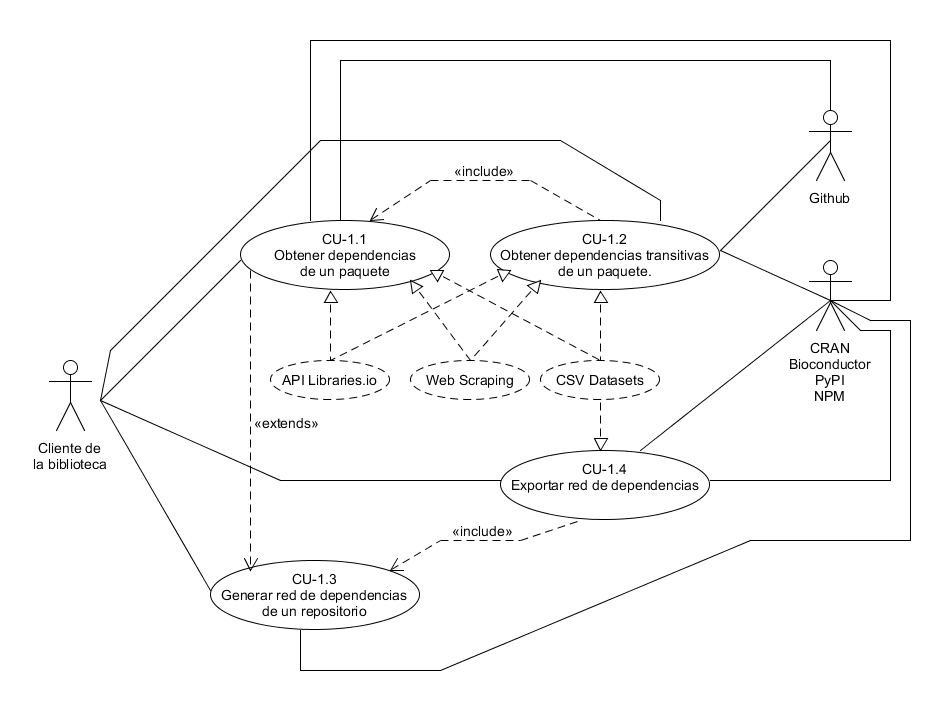
\includegraphics[width=1\textwidth]{img/anexos/CU_of.png}
	\caption{Diagrama de casos de uso de la biblioteca Olivia Finder.}
	\label{fig:casos_de_uso}
\end{figure}

Los casos de uso de la biblioteca se muestran representados en un diagrama de casos de uso en la figura \ref{fig:casos_de_uso}.
Los actores que interactúan con el sistema son el usuario y los repositorios de paquetes.

\textbf{CU-1.1: Obtener dependencias de un paquete.}

\begin{table}[p]
	\centering
	\begin{tabularx}{\linewidth}{ p{0.21\columnwidth} p{0.71\columnwidth} }
		\toprule
		\textbf{CU-1.1}               & \textbf{Obtención de las dependencias de un paquete}                              \\
		\toprule
		\textbf{Versión}              & 1.0                                                                              \\
		\textbf{Autor}                & Daniel Alonso                                                                    \\
		\textbf{Requisitos asociados} & RF-1, RF-2, RF-3, RF-6, RF-7, RF-8, RF-9                                         \\
		\textbf{Descripción}          & Obtener las dependencias de un paquete de las redes
		PyPI, npm, CRAN, Bioconductor y GitHub.                                                                          \\
		\textbf{Precondición}         & Las fuentes de datos usadas para obtener las dependencias
		deben de estar accesibles.                                                                                       \\
		\textbf{Acciones}             &
		\begin{enumerate}
			\def\labelenumi{\arabic{enumi}.}
			\tightlist
			\item Identificar el paquete del cual se desean obtener las dependencias.
			\item Realizar una búsqueda en la fuente de datos para obtener las dependencias del paquete.
		\end{enumerate}                      \\
		\textbf{Postcondición}        & Se obtienen las dependencias del paquete en formato diccionario.                 \\
		\textbf{Excepciones}          & Si el paquete no existe en alguna de las redes, se obtiene un diccionario vacío. \\
		\textbf{Importancia}          & Media                                                                            \\
		\bottomrule
	\end{tabularx}
	\caption{CU-1 Dependencias de un paquete.}
	\label{tab:cu1}
\end{table}

El caso de uso \texttt{CU-1.1} \ref{tab:cu1} se centra en la obtención de las dependencias de un paquete específico. Permite
identificar el paquete deseado y realizar una búsqueda en las fuentes de datos correspondientes, como PyPI,
npm, CRAN, Bioconductor y GitHub. Al finalizar, se obtiene un diccionario que contiene las dependencias del
paquete, lo que resulta útil para comprender las relaciones y requisitos del software.



\textbf{CU-1.2: Obtener dependencias transitivas de un paquete.}

\begin{table}[p]
	\centering
	\begin{tabularx}{\linewidth}{ p{0.21\columnwidth} p{0.71\columnwidth} }
		\toprule
		\textbf{CU-1.2}               & \textbf{Obtención de las dependencias transitivas de un paquete}                                       \\
		\toprule
		\textbf{Versión}              & 1.0                                                                                                    \\
		\textbf{Autor}                & Daniel Alonso                                                                                          \\
		\textbf{Requisitos asociados} & RF-1, RF-3, RF-7, RF-8, RF-9                                                                           \\
		\textbf{Descripción}          & Obtener las dependencias transitivas de un paquete, utilizando una profundidad de búsqueda específica. \\
		\textbf{Precondición}         & Las dependencias directas del paquete están disponibles y las fuentes de datos son accesibles.         \\
		\textbf{Acciones}             &
		\begin{enumerate}
			\def\labelenumi{\arabic{enumi}.}
			\tightlist
			\item Identificar el paquete del cual se desean obtener las dependencias transitivas.
			\item Establecer la profundidad de búsqueda deseada.
			\item Recorrer recursivamente las dependencias directas del paquete hasta alcanzar la profundidad de búsqueda establecida.
			\item Registrar todas las dependencias transitivas encontradas durante el recorrido.
		\end{enumerate}              \\
		\textbf{Postcondición}        & Se obtienen las dependencias transitivas del paquete hasta la profundidad de búsqueda especificada.    \\
		\textbf{Excepciones}          & Si el paquete no existe en las redes de paquetes, se añade como un diccionario vacío.                  \\
		\textbf{Importancia}          & Media                                                                                                  \\
		\bottomrule
	\end{tabularx}
	\caption{CU-2 Dependencias transitivas de un paquete.}
	\label{tab:cu2}
\end{table}

Por otro lado, el caso de uso \texttt{CU-1.2} \ref{tab:cu2} se enfoca en la obtención de las dependencias transitivas de un paquete.
Permite establecer una profundidad de búsqueda y recorrer de manera recursiva las dependencias directas del
paquete hasta alcanzar dicha profundidad. Durante este proceso, se registran todas las dependencias transitivas
encontradas. Esto es beneficioso para comprender el impacto y alcance de un paquete, así como las dependencias
indirectas que pueden influir en su funcionamiento.


\textbf{CU-1.3: Generar red de dependencias de un repositorio.}

\begin{table}[p]
	\centering
	\begin{tabularx}{\linewidth}{ p{0.21\columnwidth} p{0.71\columnwidth} }
		\toprule
		\textbf{CU-1.3}               & \textbf{Generación de la red de dependencias de un repositorio}                                                          \\
		\toprule
		\textbf{Versión}              & 1.0                                                                                                                      \\
		\textbf{Autor}                & Daniel Alonso                                                                                                            \\
		\textbf{Requisitos asociados} & RF-3, RF-5, RF-6, RF-7, RF-9                                                                                             \\
		\textbf{Descripción}          & Generar la red de dependencias de paquetes para un repositorio.                                                           \\
		\textbf{Precondición}         & Los repositorios PyPI, npm, CRAN y Bioconductor están accesibles via Web o disponemos de otra fuente de datos soportada. \\
		\textbf{Acciones}             &
		\begin{enumerate}
			\def\labelenumi{\arabic{enumi}.}
			\tightlist
			\item Obtener la lista de paquetes disponibles en el repositorio.
			\item Para cada paquete, obtener sus dependencias directas.
			\item Construir la red de dependencias, donde los paquetes son los nodos y las relaciones de dependencia son los enlaces.
		\end{enumerate}                                 \\
		\textbf{Postcondición}        & Se genera la red de dependencias que muestra las relaciones entre los paquetes en el repositorio.                        \\
		\textbf{Excepciones}          & Si no es posible acceder a alguno de los repositorios, se obtiene una excepción.                                         \\
		\textbf{Importancia}          & Alta                                                                                                                     \\
		\bottomrule
	\end{tabularx}
	\caption{CU-3 Red de dependencias.}
	\label{tab:cu3}
\end{table}

El caso de uso \texttt{CU-1.3} \ref{tab:cu3} se refiere a la generación de la red de dependencias de un repositorio. Este caso de uso
implica obtener la lista de paquetes disponibles en el repositorio y, para cada paquete, identificar sus
dependencias directas. Posteriormente, se construye una red de dependencias donde los paquetes son los nodos
y las relaciones de dependencia son los enlaces. Esta representación visual de las dependencias proporciona
una visión clara y estructurada de cómo los paquetes interactúan entre sí en el repositorio.



\textbf{CU-1.4: Exportar red de dependencias.}

\begin{table}[p]
	\centering
	\begin{tabularx}{\linewidth}{ p{0.21\columnwidth} p{0.71\columnwidth} }
		\toprule
		\textbf{CU-1.4}               & \textbf{Exportación de la red de dependencias}                                                                                                   \\
		\toprule
		\textbf{Versión}              & 1.0                                                                                                                                              \\
		\textbf{Autor}                & Daniel Alonso                                                                                                                                    \\
		\textbf{Requisitos asociados} & RF-3, RF-4, RF-6                                                                                                                                 \\
		\textbf{Descripción}          & Almacenar la red de dependencias para su uso posterior por otras herramientas o análisis, asegurando la compatibilidad con la biblioteca OLIVIA. \\
		\textbf{Precondición}         & Se ha generado la red de dependencias correctamente.                                                                                             \\
		\textbf{Acciones}             &
		\begin{enumerate}
			\def\labelenumi{\arabic{enumi}.}
			\tightlist
			\item Exportar la red de dependencias en un formato compatible con la biblioteca OLIVIA.
			\item Guardar el archivo de exportación en una ubicación adecuada para su uso posterior.
		\end{enumerate}                                                                                          \\
		\textbf{Postcondición}        & La red de dependencias se almacena en un formato compatible con la biblioteca OLIVIA para su posterior utilización.                              \\
		\textbf{Excepciones}          &                                                                                                                                                  \\
		\textbf{Importancia}          & Alta                                                                                                                                             \\
		\bottomrule
	\end{tabularx}
	\caption{CU-4 Exportación de la red.}
	\label{tab:cu4}
\end{table}

El caso de uso \texttt{CU-1.4} \ref{tab:cu4} se encarga de la exportación de la red de dependencias generada. Permite
almacenar la red en un formato compatible con la biblioteca \textit{OLIVIA}, asegurando su posterior utilización por
otras herramientas o análisis. Al exportar la red, se garantiza la preservación de la información sobre las
dependencias, lo que facilita su intercambio y colaboración con otros sistemas o investigadores interesados
en el análisis de paquetes y sus interconexiones.

\newpage

\subsection{Casos de uso de un cliente de la biblioteca \textit{Olivia Finder}}

\begin{figure}[ht!]
	\centering
	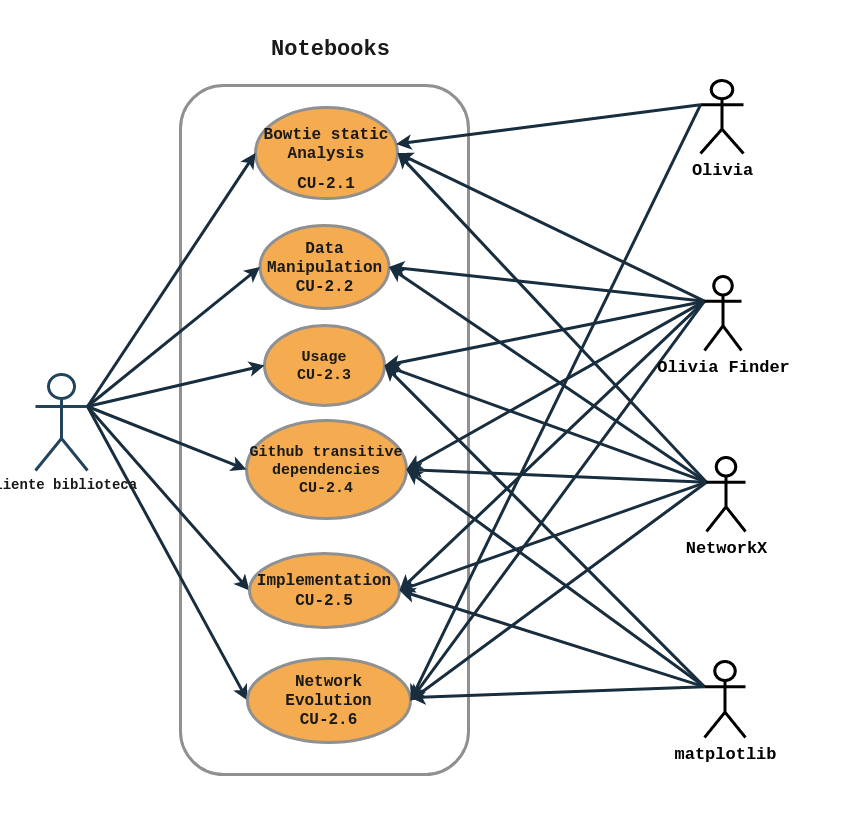
\includegraphics[width=1\textwidth]{img/anexos/CU_notebooks.png}
	\caption{Diagrama de casos de uso de los clientes de la biblioteca.}
	\label{fig:casos_de_uso_notebooks}
\end{figure}

Los casos de uso de los clientes de la biblioteca se muestran en la figura \ref{fig:casos_de_uso_notebooks}.


\textbf{CU-2.1: Análisis estático de Bow-tie.}

\begin{table}[p]
	\centering
	\begin{tabularx}{\linewidth}{ p{0.21\columnwidth} p{0.71\columnwidth} }
		\toprule
		\textbf{CU-2.1}               & \textbf{Análisis estático de Bow-tie}                                         \\
		\toprule
		\textbf{Versión}              & 1.0                                                                           \\
		\textbf{Autor}                & Daniel Alonso                                                                 \\
		\textbf{Requisitos asociados} & RF-1, RF-2, RF-3, RF-7, RF-8, RNF-1, RNF-2, RNF-4                             \\
		\textbf{Descripción}          & Realizar un análisis comparativo de las métricas
		obtenidas para conjuntos de datos utilizando una estructura de Bowtie y las métricas
		de vulnerabilidad en OLIVIA.                                                                                  \\
		\textbf{Precondición}         & Se han obtenido los conjuntos de datos y se han definido
		las métricas de vulnerabilidad en OLIVIA.                                                                     \\
		\textbf{Acciones}             &
		\begin{enumerate}
			\def\labelenumi{\arabic{enumi}.}
			\tightlist
			\item Aplicar la estructura de Bowtie a los conjuntos de datos.
			\item Calcular las métricas de vulnerabilidad definidas en OLIVIA para cada conjunto de datos.
			\item Realizar una comparativa de las métricas obtenidas.
		\end{enumerate}                 \\
		\textbf{Postcondición}        & Se obtiene un análisis comparativo de las métricas obtenidas
		para los conjuntos de datos utilizando una estructura de Bowtie y las métricas de
		vulnerabilidad en OLIVIA.                                                                                     \\
		\textbf{Excepciones}          & No se pueden obtener los conjuntos de datos o las métricas de vulnerabilidad. \\
		\textbf{Importancia}          & Alta                                                                          \\
		\bottomrule
	\end{tabularx}
	\caption{CU-2.1 Análisis estático de Bowtie.}
	\label{tab:cu2.1}
\end{table}

El \textit{Notebook} \textit{Bow-tie static analysis}\footnote{Idea sacada del artículo:
	"many directed networks show a structure where most nodes belong to a WCC that can be
	partitioned into three main subsets: the largest SCC, the set of nodes that can reach the
	SCC, i.e. the IN set, and the set of nodes that can be reached from the SCC, i.e. the OUT
	set, which is usually represented in the form of a bow-tie diagram~\cite{Broder2000309}} lleva a cabo un análisis comparativo de las
métricas obtenidas para conjuntos de datos utilizando una estructura de Bow-tie\cite{enwiki:1148363387} y
las métricas de vulnerabilidad definidas en \textit{OLIVIA}. \ref{tab:cu2.1}



\textbf{CU-2.2: Manipulación de datos.}

El caso de uso de \textit{Manipulación de datos} muestra como realizar la obtención de datos utilizando \textit{Olivia Finder}.
En concreto se muestra como se construye un objeto \texttt{PackageManager} usando las distintas fuentes de datos implementadas y cómo se pueden combinar, con el fin de obtener las dependencias
de los paquetes y entender la forma en que se presentan estos datos. \ref{tab:cu2.2}

\begin{table}[p]
	\centering
	\begin{tabularx}{\linewidth}{ p{0.21\columnwidth} p{0.71\columnwidth} }
		\toprule
		\textbf{CU-2.2}               & \textbf{Manipulación de datos}                                                      \\
		\toprule
		\textbf{Versión}              & 1.0                                                                                 \\
		\textbf{Autor}                & Daniel Alonso                                                                       \\
		\textbf{Requisitos asociados} & RF-1, RF-2, RF-3, RF-4, RF-5, RF-7, RF-9, RNF-1, RNF-2, RNF-4                       \\
		\textbf{Descripción}          & Realizar los pasos necesarios para manipular los datos
		utilizando \textit{Olivia Finder}, con el objetivo de obtener las dependencias de los
		paquetes y comprender cómo se presentan los datos.                                                                  \\
		\textbf{Precondición}         & \textit{Olivia Finder} ha sido configurado correctamente y los datos
		de los paquetes están disponibles.                                                                                  \\
		\textbf{Acciones}             & \begin{enumerate}
			                                \item Utilizar \textit{Olivia Finder} para obtener las dependencias de los paquetes.
			                                \item Analizar la forma en que se presentan los datos obtenidos.
		                                \end{enumerate} \\
		\textbf{Postcondición}        & Se comprende la forma en que se presentan los datos de las
		dependencias de los paquetes, lo que permite su posterior manipulación y análisis.                                  \\
		\textbf{Excepciones}          & No se pueden obtener las dependencias de los paquetes
		utilizando \textit{Olivia Finder}.                                                                                  \\
		\textbf{Importancia}          & Alta                                                                                \\
		\bottomrule
	\end{tabularx}
	\caption{CU-2.2 Manipulación de datos.}
	\label{tab:cu2.2}
\end{table}

\textbf{CU-2.3: Selección de estrategias de extracción de datos.}

El caso de uso \textit{Selección de estrategias de extracción de datos} presenta un procedimiento para generar un conjunto de datos
(lista de enlaces) con la red de dependencias deseada, y proporciona directrices sobre cómo
utilizarlo para realizar un análisis estático. \ref{tab:cu2.3}

\begin{table}[p]
	\centering
	\begin{tabularx}{\linewidth}{ p{0.21\columnwidth} p{0.71\columnwidth} }
		\toprule
		\textbf{CU-2.3}               & \textbf{Selección de estrategias de extracción de datos}                                                   \\
		\toprule
		\textbf{Versión}              & 1.0                                                                                                        \\
		\textbf{Autor}                & Daniel Alonso                                                                                              \\
		\textbf{Requisitos asociados} & RF-1, RF-2, RF-3, RF-7, RF-9, RNF-1, RNF-2, RNF-4                                                          \\
		\textbf{Descripción}          & Generar un conjunto de datos (lista de enlaces) con la red de dependencias
		deseada y proporcionar directrices sobre cómo utilizarlo para realizar un análisis estático.                                               \\
		\textbf{Precondición}         & Los datos de la red de dependencias y las directrices de análisis están
		disponibles.                                                                                                                               \\
		\textbf{Acciones}             & \begin{enumerate}
			                                \item Generar un conjunto de datos (lista de enlaces) que represente la red de dependencias deseada.
			                                \item Proporcionar directrices sobre cómo utilizar el conjunto de datos para realizar un análisis estático.
		                                \end{enumerate} \\
		\textbf{Postcondición}        & Se dispone de un conjunto de datos que representa la red de dependencias
		deseada y se conocen las directrices para realizar un análisis estático utilizando dicho
		conjunto.                                                                                                                                  \\
		\textbf{Excepciones}          & No se pueden generar los datos de la red de dependencias o las
		directrices de análisis están ausentes o incorrectas.                                                                                      \\
		\textbf{Importancia}          & Alta                                                                                                       \\
		\bottomrule
	\end{tabularx}
	\caption{CU-2.3 Uso.}
	\label{tab:cu2.3}
\end{table}

\textbf{CU-2.4: Dependencias transitivas de un repositorio de GitHub.}

El caso de uso de \textit{Dependencias transitivas de un repositorio de GitHub} está diseñado para obtener las dependencias transitivas de un repositorio
en \textit{GitHub}. Se basa en una exploración exhaustiva de las dependencias de un paquete,
alcanzando la profundidad deseada en el árbol de dependencias. \ref{tab:cu2.4}

\begin{table}[p]
	\centering
	\begin{tabularx}{\linewidth}{ p{0.21\columnwidth} p{0.71\columnwidth} }
		\toprule
		\textbf{CU-2.4}               & \textbf{Dependencias transitivas de un repositorio de GitHub}                                                                                                              \\
		\toprule
		\textbf{Versión}              & 1.0                                                                                                                                                                        \\
		\textbf{Autor}                & Daniel Alonso                                                                                                                                                              \\
		\textbf{Requisitos asociados} & RF-1, RF-2, RF-3, RF-4, RF-5, RF-7, RF-9, RNF-1, RNF-2, RNF-4                                                                                                              \\
		\textbf{Descripción}          & Obtener las dependencias transitivas de un repositorio en GitHub mediante una exploración exhaustiva de las dependencias de un paquete, alcanzando la profundidad deseada. \\
		\textbf{Precondición}         & Se ha especificado el repositorio objetivo y se ha definido la profundidad deseada para la exploración de dependencias.                                                    \\
		\textbf{Acciones}             & \begin{enumerate}
			                                \item Identificar el repositorio objetivo en GitHub.
			                                \item Realizar una exploración exhaustiva de las dependencias del paquete, alcanzando la profundidad deseada en el árbol de dependencias.
			                                \item Registrar las dependencias transitivas obtenidas.
		                                \end{enumerate}                                   \\
		\textbf{Postcondición}        & Se obtienen las dependencias transitivas del repositorio objetivo, registradas y listas para su análisis posterior.                                                        \\
		\textbf{Excepciones}          & No se puede acceder al repositorio en GitHub o no se encuentran las dependencias del paquete en el repositorio.                                                            \\
		\textbf{Importancia}          & Alta                                                                                                                                                                       \\
		\bottomrule
	\end{tabularx}
	\caption{CU-2.4 Dependencias transitivas de GitHub.}
	\label{tab:cu2.4}
\end{table}


\textbf{CU-2.5: Detalles de implementación (Para programadores).}

Este caso de uso, pese a ser muy genérico proporciona una guía detallada para desarrolladores sobre la implementación
de la herramienta, mostrando las funcionalidades de los distintos módulos. Ofrece una visión en
profundidad de la biblioteca y sus componentes. Está pensado introducir de una forma descriptiva el funcionamiento de la biblioteca
a un nivel más bajo y ser de ayuda para el programador que decida hacer reimplementaciones de la biblioteca. \ref{tab:cu2.5}

\begin{table}[p]
	\centering
	\begin{tabularx}{\linewidth}{ p{0.21\columnwidth} p{0.71\columnwidth} }
		\toprule
		\textbf{CU-2.5}               & \textbf{Implementación}                                                                                                                              \\
		\toprule
		\textbf{Versión}              & 1.0                                                                                                                                                  \\
		\textbf{Autor}                & Daniel Alonso                                                                                                                                        \\
		\textbf{Requisitos asociados} & RF-1, RF-2, RF-3, RF-4, RF-5, RF-6, RF-7, RF-8, RF-9, RNF-1, RNF-2, RNF-3, RNF-4, RNF-5                                                              \\
		\textbf{Descripción}          & Proporcionar una guía detallada para el desarrollador sobre la implementación de la herramienta, mostrando las funcionalidades de los módulos.       \\
		\textbf{Precondición}         & Se ha realizado la implementación de la herramienta y se dispone de los módulos correspondientes.                                                    \\
		\textbf{Acciones}             & \begin{enumerate}
			                                \item Describir las funcionalidades de los módulos de la herramienta.
			                                \item Explicar el uso adecuado de cada módulo y sus componentes.
			                                \item Proporcionar ejemplos de código para ilustrar la implementación.
		                                \end{enumerate}                                                                                \\
		\textbf{Postcondición}        & El desarrollador obtiene una visión en profundidad de la biblioteca y sus componentes, lo que facilita la implementación y el uso de la herramienta. \\
		\textbf{Excepciones}          & Problemas en la herramienta o faltan los módulos correspondientes.                                                                                   \\
		\textbf{Importancia}          & Alta                                                                                                                                                 \\
		\bottomrule
	\end{tabularx}
	\caption{CU-2.5 Implementación.}
	\label{tab:cu2.5}
\end{table}

\textbf{CU-2.6: Evolución de la red.}

El caso de uso de \textit{Evolución de la red} presentan un análisis evolutivo de los repositorios
desde una perspectiva experimental. Se realiza un análisis gráfico
básico de cómo ha variado el repositorio a lo largo del tiempo, utilizando los datos
de \textit{Libraries.io}\cite{jeremy_katz_2020_3626071} del año 2020 y los datos obtenidos mediante \textit{Olivia Finder} en el 2023. \ref{tab:cu2.6}


\begin{table}[p]
	\centering
	\begin{tabularx}{\linewidth}{ p{0.21\columnwidth} p{0.71\columnwidth} }
		\toprule
		\textbf{CU-2.6}               & \textbf{Evolución de la red}                                                                                                                                                              \\
		\toprule
		\textbf{Versión}              & 1.0                                                                                                                                                                                       \\
		\textbf{Autor}                & Daniel Alonso                                                                                                                                                                             \\
		\textbf{Requisitos asociados} & RF-1, RF-4, RF-7, RF-9, RNF-1, RNF-2, RNF-4, RNF-5                                                                                                                                        \\
		\textbf{Descripción}          & Realizar un análisis evolutivo de los repositorios desde una perspectiva experimental, proporcionando un análisis gráfico básico de cómo ha variado el repositorio a lo largo del tiempo. \\
		\textbf{Precondición}         & Se disponen de los datos de \textit{Libraries.io} del año 2020 y de los datos obtenidos mediante \textit{Olivia Finder}.                                                                  \\
		\textbf{Acciones}             & \begin{enumerate}
			                                \item Utilizar los datos de \textit{Libraries.io} y de \textit{Olivia Finder} para analizar la evolución de los repositorios.
			                                \item Generar gráficos que ilustren cómo ha variado el repositorio a lo largo del tiempo.
			                                \item Realizar un análisis comparativo de los resultados obtenidos.
		                                \end{enumerate}                                                              \\
		\textbf{Postcondición}        & Se obtiene un análisis evolutivo de los repositorios, que proporciona una visión básica de cómo ha variado el repositorio a lo largo del tiempo.                                          \\
		\textbf{Excepciones}          & No se disponen de los datos de \textit{Libraries.io} del año 2020 o de los datos obtenidos mediante \textit{Olivia Finder}.                                                               \\
		\textbf{Importancia}          & Alta                                                                                                                                                                                      \\
		\bottomrule
	\end{tabularx}
	\caption{CU-2.6 Evolución de la red.}
	\label{tab:cu2.6}
\end{table}


\section{Objetivos generales}

Los objetivos generales de este Trabajo de Fin de Grado se centran en la obtención de conjuntos de
datos de los repositorios de software \textit{CRAN}, \textit{Bioconductor}, \textit{PyPI} y \textit{npm},
con el propósito de generar redes de dependencias de paquetes.

Estos objetivos se concretan en el desarrollo de la biblioteca \textit{Olivia Finder}, una herramienta
que permite la adquisición de datos, manipulación y exportación en formatos compatibles con la
biblioteca \textit{OLIVIA} y otras bibliotecas de análisis de redes, como \textit{NetworkX}.

Con el fin de obtener una visión más completa de la red de dependencias de los repositorios
seleccionados, se incluirán análisis evolutivos que reflejen los estados y cambios en dichos repositorios.
Estos análisis proporcionarán información sobre el tamaño, distribución de grado y otras métricas de
centralidad relevantes para los paquetes presentes en los repositorios.

Además, se lleva a cabo un esfuerzo en la descripción del funcionamiento de la biblioteca, con el objetivo 
de asegurar su mantenimiento y continuidad en el desarrollo, mejoras y ampliación de funcionalidades. Se 
documentan \textit{funcionalidades}, \textit{estructuras de datos} y \textit{flujos de trabajo}. Se destaca 
la importancia de mantener una arquitectura modular, lo que facilita la incorporación 
de nuevas características sin afectar la estabilidad general del sistema. Asimismo, se establecen estándares 
de codificación y buenas prácticas para asegurar la legibilidad del código y favorecer la colaboración entre 
desarrolladores. La documentación resultante actúa como un recurso valioso para el equipo de desarrollo y 
la comunidad de usuarios para mantener con vida la biblioteca.

% \section{Catálogo de requisitos}

% \section{Especificación de requisitos}






\apendice{Especificación de diseño}

\section{Introducción}

\section{Diseño de datos}

\subsection{Estructuras de datos}
La información relativa a la red de dependencias de paquetes se almacena en un formato híbrido 
que contiene varias estructuras de datos con distintos objetivos:

\begin{itemize}
\item Almacenar la información concreta de paquetes y dependencias del repositorio, en un formato 
que permita realizar de forma eficiente las operaciones más comunes relacionadas con el objeto 
de la biblioteca.

\item Ser capaz de aceptar extensibilidad por si en un determinado momento hubiese que ampliar 
o variar los datos que almacenamos.
\end{itemize}
\

De esta forma, representamos cada paquete mediante una estructura de datos específica para 
contener los atributos que deseamos representar. La red de dependencias queda representada 
como un diccionario de paquetes. Esta representación permite acceder a un paquete de forma 
eficiente, lo cual resulta importante para el correcto funcionamiento de la herramienta.

\subsection{Datos de entrada}

Podemos construir la red de dependencias a través de un fichero CSV que represente la lista 
de enlaces. Los paquetes se pueden reconstruir a partir de una estructura tipo diccionario 
con los atributos implementados. Las listas de paquetes se dan en formato lista de objetos 
paquete.

Un problema que se ve es la redundancia de los nombres de nodos, pero realmente es necesario 
si queremos almacenar datos más concretos sobre la relación de dependencia, como la versión 
concreta de una dependencia que usa un paquete, etc.

\subsection{Datos de salida}
La red se puede exportar a formato de grafo dirigido de \textit{NetworkX} y también como 
un diccionario de listas de dependencias.

La estructura de datos \textit{Paquete} se puede exportar como un diccionario, mientras 
que un conjunto de paquetes se exportará como una lista de objetos \textit{paquetes}.

\subsection{Ficheros de entrada}
Podemos emplear un archivo CSV como fuente de datos.

Podemos emplear objetos serializados de tipo \textit{PackageManager}.

\subsection{Ficheros de salida}
Podemos generar ficheros \textit{CSV} con la representación de la red o exportarlo como un dataframe de \textit{Pandas},
lo que nos permite exportarlo a otros formatos como \textit{JSON, HTML, etc}.

También podemos realizar un exportado mediante la serialización del objeto \textit{PackageManager} 
como estructura global de persistencia para un repositorio. Este tipo de archivo se le ha dado una 
extensión \textit{.olvpm} para poder identificarlo correctamente.

\section{Diseño procedimental}

\subsection{Modulo olivia\_finder.package}

\textit{Package} es uno de los módulos base de \textit{olivia-finder}, cuya funcionalidad radica en 
constituir una estructura de datos que contiene la representación del paquete. Está compuesto por 
atributos en formato \textit{string} y una lista de dependencias (\textit{lista de objetos paquete}).

En nuestra implementación, los atributos que almacenamos son el nombre, la versión, la URL y las 
dependencias. Las principales funcionalidades que implementa son la representación como un 
diccionario, la carga a partir de una estructura de tipo diccionario y la enumeración de las 
dependencias.


\subsection{Modulo olivia\_finder.package\_manager}

El módulo \textit{Package Manager} es un wrapper de los datos que conforman la red de dependencias de
 un repositorio y de la funcionalidad del objeto \textit{DataSource}, que representa la fuente de 
 datos de un repositorio. Aporta funcionalidades para la carga, obtención y persistencia de los datos.

Para inicializar el objeto, necesitamos pasarle como argumento una lista de los \textit{data sources} 
que deseemos usar. Está pensado para tener como mínimo un \textit{data source} principal y una serie 
de \textit{data sources} auxiliares opcionales, donde se realizará la búsqueda si no se obtiene un 
resultado mediante el principal.

Respecto a la carga de datos en sus estructuras, podemos emplear ficheros de 
persistencia \textit{.olvpm} o archivos CSV con la lista de enlaces.

La obtención de datos se puede realizar de forma individual para un paquete o para una lista de 
paquetes. Una vez obtenidos los datos, si se desea, se pueden almacenar en la estructura interna 
de la clase, que es un diccionario, y recuperarlos desde ahí. Por lo tanto, si queremos usar los 
datos directamente desde las estructuras de la clase, primero debemos inicializar los datos.

Una funcionalidad interesante es la obtención de redes de dependencias transitivas a partir de un 
paquete y dada una profundidad de búsqueda.

La exportación de los datos se puede representar mediante un objeto diccionario de nodos que 
contienen listas de nombres de paquetes, es decir, una lista de adyacencia. El principal formato 
de exportación que vamos a tratar son los archivos CSV en formato lista de enlaces, debido a su 
naturaleza legible y su integración con OLIVIA. También es interesante su representación como 
grafo dirigido de \textit{NetworkX} (\textit{nx.DiGraph}).

La persistencia de los datos se lleva a cabo mediante la serialización del objeto utilizando el 
módulo \textit{pickle} de Python, o la generación de archivos CSV de lista de enlaces.

Se incorporan excepciones características para representar los problemas más comunes en un contexto 
más descriptivo sobre la actuación de la herramienta.

\subsection{Paquete olivia\_finder.utilities}

El paquete \textit{utilities} contiene un conjunto de módulos que implementan funcionalidades de 
utilidad para la aplicación, aunque no forman parte central de ella. Está compuesto por los siguientes módulos:

El módulo \textit{config} implementa una funcionalidad para la carga de la configuración 
definida en el archivo \textit{config.ini}\footnote{Archivo de configuracion de la biblioteca}, donde se especifican las configuraciones necesarias.

El módulo \textit{exception} implementa una excepción genérica para la herramienta, que 
puede ser utilizada para capturar y manejar situaciones excepcionales.

El módulo \textit{logger} implementa funcionalidades para llevar un registro de los 
eventos ocurridos durante la ejecución de la aplicación.

El módulo \textit{singleton\_decorator} implementa un patrón de diseño singleton basado 
en el decorador, que se puede aplicar a cualquier clase para garantizar que solo se cree una 
única instancia de dicha clase.

El módulo \textit{utilities} proporciona algunas funcionalidades concretas y frecuentemente 
utilizadas en la aplicación.

\subsection{Paquete olivia\_finder.myrequests}

Este paquete implementa la funcionalidad de realizar \textit{peticiones web} de forma concurrente 
y mediante rotación de \textit{proxies} y \textit{user agents} para ocultar la identidad del realizador
 de la petición.

Está compuesto por los siguientes módulos y paquetes:

El módulo \textit{proxy\_handler} se encarga de gestionar los proxies que se utilizarán para 
realizar las peticiones. Lleva un control del número de usos de cada proxy y gestiona su rotación 
para evitar la repetición en peticiones concurrentes. Además, obtiene nuevos proxies cuando ha 
agotado los existentes. Implementa el patrón de diseño \textit{singleton}.

El paquete \textit{proxy\_builders} implementa la funcionalidad de obtención de una lista de 
proxies de Internet. La funcionalidad está descrita en la clase abstracta \textit{ProxyBuilder} del moulo \textit{proxy\_builders}, 
que se encarga de implementar las funcionalidades comunes y sirve como interfaz para las distintas 
clases que implementan \textit{ProxyBuilder}. Estas clases se encuentran en los
 módulos \textit{list\_builder} y \textit{ssl\_proxies}.

El módulo \textit{proxy\_builders.list\_builder} se encarga de obtener una lista de proxies almacenada en un
 servidor web en formato \textit{txt}.

El módulo \textit{proxy\_builders.ssl\_proxies} realiza la misma función, pero obtiene los datos de los 
proxies mediante \textit{web scraping} de un sitio web que ofrece este servicio.

El módulo \textit{useragent\_handler} realiza una función similar al 
módulo \textit{proxy\_handler}, pero con los \textit{user agents}. Implementa la obtención a 
través de un archivo estático que contiene una lista de \textit{user agents} y también mediante \textit{web scraping} de una página web que contiene un listado. Gestiona la rotación de los \textit{user agents} para evitar su repetición. También implementa el patrón de diseño \textit{singleton}.

El módulo \textit{job} es un \textit{wrapper} de los atributos de una petición web. 
Encapsula la URL de destino, los parámetros de la petición y almacena la respuesta del servidor.

El módulo \textit{request\_worker}, que hereda de la clase \textit{Thread}, se encarga de 
realizar las peticiones web asignadas a él.

Por último, el módulo \textit{request\_handler} implementa toda la lógica del 
paquete \textit{myrequests}. Se encarga de gestionar los trabajos de petición web a realizar y 
asignarlos a los \textit{workers}, que se encargan de realizar estas peticiones de forma concurrente. 
Recoge los trabajos realizados y los devuelve.

Estos módulos y paquetes en conjunto permiten realizar peticiones web de forma eficiente, 
garantizando la anonimización del realizador de la petición mediante el uso de proxies y user 
agents rotativos.

\subsection{Paquete olivia\_finder.data\_source}

Este paquete implementa la funcionalidad de obtención de datos desde distintas fuentes.

En primer lugar, tenemos el módulo \textit{data\_source} que implementa una clase abstracta que 
sirve como interfaz para las distintas clases de este paquete. Un \textit{data source} debe implementar
 la lógica de obtención de una lista de paquetes disponibles y la obtención de los datos de los paquetes.

Tenemos 3 módulos que implementan \textit{DataSource}:

El módulo \textit{data\_source}.\textit{scraper\_ds} implementa la obtención de datos de los paquetes 
mediante \textit{web scraping} y proporciona una interfaz para las implementaciones concretas
 de \textit{scraper} para los repositorios de software. Las funcionalidades que aporta incluyen 
 la generación y lanzamiento de trabajos de petición web correspondientes a la obtención de los datos 
 de los paquetes, así como la recolección de los datos de estas peticiones.

Las implementaciones concretas del módulo \textit{repository\_scrapers}.\textit{scraper\_ds} se encuentran 
dentro del subpaquete \textit{repository\_scrapers}, el cual contiene los módulos \textit{repository\_scrapers}.\textit{bioconductor},
\textit{repository\_scrapers}.\textit{cran}, \textit{repository\_scrapers}.\textit{npm} 
y \textit{repository\_scrapers}.\textit{pypi}, que realizan la labor descrita para cada uno de 
estos repositorios. Además, incluye el módulo \textit{repository\_scrapers}.\textit{github}, que permite 
realizar una labor similar a través de la sección \textit{Insights > Dependency graph > Dependencies}, que se puede 
habilitar en un repositorio de GitHub.

El módulo \textit{data\_source}.\textit{csv\_ds} proporciona soporte para usar un dataset en formato CSV como fuente de 
datos. La funcionalidad que ofrece es similar a la mencionada anteriormente, pero adaptada y optimizada 
para este tipo de archivo.

El módulo \textit{data\_source}.\textit{librariesio\_ds} realiza la misma función que los anteriores, pero utiliza la 
API de \textit{data\_source}.\textit{libraries.io}. No todas las funcionalidades han podido ser implementadas en este 
módulo, por ejemplo, la lista de paquetes de un repositorio no está soportada. Sin embargo, ofrece 
un conjunto de datos más amplio al acceder directamente al conjunto de datos de \textit{libraries.io} 
a través de su API. Para poder utilizar esta funcionalidad, es necesario disponer de una clave de API 
de \textit{libraries.io}.

\section{Diseño arquitectónico}

La arquitectura de la herramienta se basa en un enfoque modular y bien estructurado que permite la 
representación y manipulación eficiente de la red de dependencias de paquetes de un repositorio. La aplicación se 
compone de varios módulos y paquetes que trabajan en conjunto para obtener, procesar y persistir los datos. 
Cada módulo tiene responsabilidades específicas y se comunica con otros módulos a través de interfaces definidas. 
El diseño de datos se centra en la representación de paquetes y dependencias utilizando estructuras de datos 
adecuadas, como diccionarios y listas. La aplicación también implementa patrones de diseño, como el patrón singleton, 
para garantizar la creación de instancias únicas y la reutilización de recursos. A continuación, se presentarán 
los diagramas de clase de cada módulo o paquete para proporcionar una visión más detallada de la arquitectura de 
la aplicación.
\apendice{Documentación técnica de programación}

\section{Introducción}
Se recoge en este apartado la información más relevante para la extensión
o adaptación del código de la biblioteca.

\section{Estructura de directorios}
El proyecto de software está disponible en el repositorio público\footnote{\url{https://github.com/dab0012/olivia-finder}}.
Este repositorio incluye los objetos de persistencia, los datos extraídos en los análisis y todo el
conjunto de scripts y demás material utilizado. Sin embargo, si lo que le interesa son los datos generados de las redes de dependencias,
es recomendable acceder a ellos desde los siguientes mirrors en \textit{Zenodo}.\footnote{\url{https://zenodo.org/record/8095863}}.

EL conjunto de datos completo usado en los experimentos esta disponble en \textit{Kaggle}.\footnote{\url{https://www.kaggle.com/datasets/danielalonsob/dependency-networks}}

\subsection{Estructura de directorios del repositorio}

El repositorio alberga una amplia gama de contenido, que incluye tanto la biblioteca Olivia-Finder que hemos
desarrollado como la biblioteca \textit{OLIVIA} realizada en el anterior Trabajo de Fin de Grado. Además, se encuentra
disponible documentación detallada sobre ambas bibliotecas, que proporciona información exhaustiva sobre su
funcionamiento y características.

Dentro del repositorio, también se pueden encontrar una serie de notebooks que ofrecen demostraciones interactivas
de la funcionalidad de las bibliotecas. Estos notebooks permiten a los usuarios explorar y experimentar con los
datos generados por las redes que hemos creado, lo que facilita la comprensión y el análisis de los resultados
obtenidos.

Además del código y la documentación, el repositorio cuenta con una variedad de material auxiliar, como scripts
y funcionalidades adicionales. Estos recursos complementarios ofrecen soporte adicional para aquellos interesados
en ampliar o personalizar las funcionalidades de las bibliotecas.

\begin{verbatim}
    olivia_finder
    |-- docs
    |-- notebooks
    |   |-- common
    |   |-- olivia
    |   |-- olivia_finder
    |   |-- resources
    |   `-- results
    |       |-- csv_datasets
    |       |-- network_models
    |       |-- package_lists
    |       `-- package_managers
    |-- olivia
    |   |-- docs
    |   `-- olivia
    `-- olivia_finder
        |-- diagrams
        `-- olivia_finder
    \end{verbatim}


Sobre la raiz del repositorio, se encuentra el directorio \textit{docs} contiene la documentación de la biblioteca, mientras que el directorio \textit{notebooks}
contiene los notebooks que ofrecen demostraciones interactivas de las bibliotecas.

Dentro de \textit{notebooks}, el directorio \textit{common} contiene notebooks que ofrecen funcionalidades comunes
a ambas bibliotecas, mientras que los directorios \textit{olivia} y \textit{olivia\_finder} contienen notebooks
que ofrecen funcionalidades específicas de cada biblioteca.
El directorio \textit{resources} contiene los algun scripts
y recursos adicionales de utilidad. Por último, el directorio \textit{results} contiene los datos generados por las
redes de dependencias, que se encuentran organizados en subdirectorios según su tipo.

En la raiz del repositorio, se encuentran los directorios \textit{olivia} y \textit{olivia\_finder}, que contienen
las bibliotecas \textit{OLIVIA} y Olivia-Finder, respectivamente. Dentro de cada uno de estos directorios, se encuentra
el directorio \textit{olivia} o \textit{olivia\_finder}, que contienen el código de las bibliotecas.


\section{Manual del programador}

\subsection{Entrorno de desarrollo}

El proyecto puede descargarse directamente o clonarse desde el repositorio \footnote{\url{https://github.com/dab0012/olivia-finder}}
con \texttt{git}. Ha sido desarrollado en \texttt{python3.11} buscando la compatibilidad con \texttt{python3.8} por
ser la máxima versión soportada por la librería \textit{OLIVIA}.
Las dependencias de la biblioteca se especifican en el archivo \texttt{requirements.txt}:


\textbf{Manejo de datos:}
\begin{itemize}
    \item \texttt{pandas}
    \item \texttt{networkx}
\end{itemize}

\textbf{Obtención de datos:}
\begin{itemize}
    \item \texttt{requests}
    \item \texttt{BeautifulSoup4}
    \item \texttt{selenium}
    \item \texttt{pybraries}
\end{itemize}

\textbf{Utilidad extra:}
\begin{itemize}
    \item \texttt{tqdm}
    \item \texttt{typing\_extensions}
\end{itemize}

En el caso de querer hacer un uso combinado de la biblioteca \textit{Olivia Finder} y \textit{OLIVIA}, se recomienda el uso de entornos
virtuales de Python para facilitar el despliegue. Se debe crear un entorno de la versión de \textit{Python3.8} e instalar los
requisitos de la biblioteca \textit{OLIVIA} en primer lugar debido a la necesidad de esta de versiones concretas de sus
dependencias, en concreto:

\begin{center}

    \texttt{intbitset==2.4.0}

    \texttt{numpy==1.18.5}

    \texttt{networkx==2.4}

\end{center}

La forma más sencilla de instalar los paquetes en el entorno es mediante el gestor de paquetes \texttt{pip} usando el
comando para cada biblioteca:

\begin{center}
    \texttt{pip install -r requirements.txt}
\end{center}

\subsection{Documentación para el programador}

Se recogen a continuación los principales recursos documentales necesarios para el desarrollo o extensión de la biblioteca \textit{Olivia Finder}:

\textbf{Documentación de la API de \textit{Olivia Finder}}:
\begin{itemize}
\item Disponible en la carpeta \textbackslash docs y accesible en línea a través de la página de Github: 

\url{https://dab0012.github.io/olivia-finder}
\end{itemize}

\textbf{Documentación de los paquetes}:
\begin{itemize}
\item Documentación de pandas:

\url{https://pandas.pydata.org/}
\item Documentación de tqdm:
 
\url{https://tqdm.github.io/}
\item Documentación de requests:
 
\url{https://docs.python-requests.org/}
\item Documentación de BeautifulSoup4:
 
\url{https://www.crummy.com/software/BeautifulSoup/bs4/doc/}
\item Documentación de selenium: 
 
\url{https://www.selenium.dev/documentation/en/}
\item Documentación de networkx: 
 
\url{https://networkx.org/documentation/stable/}
\item Documentación de matplotlib: 
 
\url{https://matplotlib.org/stable/contents.html}
\item Documentación de pybraries: 
 
\url{https://pybraries.readthedocs.io/}
\item Documentación de typing\_extensions: 
 
\url{https://typing-extensions.readthedocs.io/}
\end{itemize}

Como anexo, introducimos también la documentación de \textit{OLIVIA}:

\begin{itemize}
\item Documentación de la API: Disponible en la carpeta \textbackslash docs y accesible en línea a través de la página de Github: 

\url{https://dsr0018.github.io/olivia}
\item Documentación de NetworkX 2.4: 

\url{https://networkx.org/documentation/networkx-2.4.D.3}
\item Documentación de NumPy 1.18: 

\url{https://numpy.org/doc/1.18/}
\item Documentación de intbitset: 

\url{https://intbitset.readthedocs.io/en/latest/}
\end{itemize}

\section{Compilación, instalación y ejecución del proyecto}

El código de la biblioteca esta escrito en Python y debido a las caracteristicas de este lenguaje de programación
no requiere un paso de compilación explícita. Dadas por 
satisfechas las dependencias especificadas en \textit{requirements.txt}, los módulos pueden importarse 
en el proyecto actual como cualquier otro módulo Python.

No obstante, determinadas funcionalidades, como aquellas que requieren el uso de \textit{la API de libraries.io}, 
dependen de la \textit{API key} proporcionada por los proveedores del servicio. Esta \textit{API key} 
debe ser configurada en el archivo de configuración \textit{config.ini} en la raíz de la carpeta de 
código de la biblioteca. Desde este mismo archivo, también podemos configurar el sistema de logs de 
la herramienta.

\section{Pruebas del sistema}

Las pruebas del correcto funcionamiento del sistema se establecen mediante una serie de \textit{notebooks de demostración} 
que abarcan tanto la funcionalidad como el uso de la aplicación, los cuales comentamos en la seccion de documentacion de usuario. Estos notebooks permiten verificar exhaustivamente el 
comportamiento del sistema en diferentes escenarios y validar su conformidad con los requisitos establecidos.

Dado que no existe un método de validación preciso que nos permita determinar si el conjunto de datos utilizado es fiel a 
la realidad, se asume inicialmente que los datos son más exactos y actualizados en comparación con los proporcionados por 
\textit{libraries.io}. Esta percepción se basa en el \textit{aumento del número de paquetes} en el período temporal que 
separa ambos conjuntos de datos, así como en la aparente \textit{evolución de las relaciones de dependencia} de manera esperada.

\section{Documentación del código fuente}

La biblioteca Olivia Finder ha sido desarrollada con comentarios docstring en formato 
\textit{numpydoc}\footnote{\url{https://numpydoc.readthedocs.io/en/latest/}}, 
el cual sigue las convenciones de documentación de \textit{NumPy} y es compatible con \textit{Sphinx}\footnote{\url{https://www.sphinx-doc.org/}} y otros generadores 
automáticos de documentación. Estos comentarios docstring proporcionan descripciones detalladas de 
las clases, métodos y funciones, así como información sobre los parámetros, tipos de retorno y ejemplos 
de uso. Esto facilita la comprensión y el uso correcto de la biblioteca por parte de los desarrolladores.

Para convertir los docstrings en otros formatos, como reStructuredText o Markdown, se puede utilizar la 
herramienta Pyment\footnote{\url{https://github.com/dadadel/pyment/blob/master/doc/sphinx/source/pyment.rst}}. \textit{Pyment} es una utilidad de línea de comandos 
que permite extraer y convertir los comentarios docstring de un código fuente Python a diferentes formatos 
de documentación. Su flexibilidad y capacidad de personalización lo convierten en una herramienta útil 
para adaptar la documentación a las necesidades específicas del proyecto.

Por otro lado, la documentación publicada en el repositorio de la biblioteca Olivia Finder ha sido generada 
con \textit{pdoc}\footnote{\url{https://pdoc3.github.io/pdoc/}}. \textit{Pdoc} es una herramienta de generación de documentación 
para proyectos Python que se enfoca en la simplicidad y la facilidad de uso. Al ejecutar el comando:

\begin{center}
    \texttt{pdoc -html -o docs olivia}
\end{center}

se genera la documentación en formato HTML y se almacena en la 
carpeta \texttt{docs}. Esta documentación incluye descripciones de módulos, clases, métodos y funciones,
 así como ejemplos de uso y referencias cruzadas entre elementos de la biblioteca.

Es importante destacar que dentro de la carpeta \texttt{docs} se proporciona el script \texttt{build.sh}, 
el cual automatiza el proceso de generación de la documentación. Al ejecutar este script, se realiza la 
generación de la documentación de forma rápida y sencilla, asegurando la disponibilidad de una documentación 
actualizada y coherente para los usuarios de la biblioteca.
\apendice{Documentación de usuario}

\section{Introducción}

Se detallan a continuación las referencias necesarias para la instalación y utilización de la biblioteca.

\section{Requisitos de usuarios}

Para el correcto funcionamiento del sistema, se establecen una serie de requisitos indispensables.
En primer lugar, se requiere disponer de una \textit{conexión a internet} estable, lo cual permitirá el
acceso y uso de las funcionalidades ofrecidas.

Se necesita instalar las \textit{dependencias} necesarias de la biblioteca a partir del archivo \textit{requirements.txt},
mediante la utilización de un gestor de paquetes como \textit{pip}.

Adicionalmente, para garantizar el funcionamiento, se requiere disponer de \textit{Python} en su versión
3.8 o superior, lo cual asegurará una compatibilidad adecuada con el sistema y sus funcionalidades.

Cabe destacar que en caso de desechar la ejecución de los \textit{notebooks}, es posible que se deban
satisfacer ciertas dependencias adicionales a la biblioteca principal. Estas dependencias, aunque opcionales,
deberán ser satisfechas individualmente por cada usuario, según sus necesidades y preferencias específicas.

\section{Instalación}

El repositorio presenta una estructura bien definida que establece las ubicaciones de los recursos utilizados por los cuadernos,
scripts y otros elementos. Se recomienda encarecidamente respetar esta estructura durante el uso del repositorio, ya que esto
asegurará un funcionamiento óptimo y coherente.

Sin embargo, es importante destacar que existe la posibilidad de personalizar la ubicación de la carpeta de código de la
biblioteca (\textit{olivia\_finder/olivia\_finder}) si se configura correctamente la variable de entorno \texttt{PYTHONPATH}
para que apunte a la biblioteca. Esto permite una mayor flexibilidad en el desarrollo y la organización del proyecto.

A continuación se muestra una propuesta de estructura de directorios que podría ser utilizada en un entorno de desarrollo:

\begin{verbatim}
    .
    |-- olivia_finder               # Biblioteca
    |   |-- config.ini
    |   |-- data_source
    |   |-- __init__.py
    |   |-- myrequests
    |   |-- package_manager.py
    |   |-- package.py
    |   `-- utilities
    |-- requirements.txt            # Dependencias
    `-- test_package_manager.py     # Script de demostración
    
\end{verbatim}

En esta estructura, el directorio principal del proyecto contiene la carpeta \textit{olivia\_finder}, que incluye
los archivos y módulos relevantes para la biblioteca. Además, se encuentra el archivo \textit{config.ini} para la configuración.

Además, se incluyen los archivos \textit{requirements.txt} y \textit{test\_package\_manager.py}, que son de utilidad
para gestionar las dependencias y realizar una demostración básica de funcionamiento de la biblioteca, respectivamente.

\section{Manual del usuario}

Con el fin de adquirir una comprensión más profunda sobre las capacidades y aplicaciones de la biblioteca,
se sugiere acceder a los notebooks de demostración de funcionalidad que han sido preparados:


\begin{itemize}
    \item \textbf{Olivia Finder - Data manipulation.ipynb}\footnote{\url{https://github.com/dab0012/olivia-finder/blob/master/notebooks/olivia_finder/Olivia\%20Finder\%20-\%20Data\%20manipulation.ipynb}}:
          Este cuaderno de demostración aborda la manipulación de datos y presenta diversas funcionalidades ofrecidas por la biblioteca.
    \item \textbf{Olivia Finder - Github repository example.ipynb}\footnote{\url{https://github.com/dab0012/olivia-finder/blob/master/notebooks/olivia_finder/Olivia\%20Finder\%20-\%20Github\%20repository\%20example.ipynb}}:
          En este cuaderno, se proporciona un ejemplo práctico de cómo utilizar la biblioteca Olivia Finder para interactuar con repositorios de GitHub y extraer información relevante.
    \item \textbf{Olivia Finder - Usage.ipynb}\footnote{\url{https://github.com/dab0012/olivia-finder/blob/master/notebooks/olivia_finder/Olivia\%20Finder\%20-\%20Usage.ipynb}}:
          Este cuaderno de uso brinda una visión general de las funcionalidades de la biblioteca.
\end{itemize}

\newpage

A continuación, se expone un fragmento de código en lenguaje Python que ejemplifica un procedimiento
para la adquisición de datos provenientes del repositorio de paquetes \textit{CRAN}.

\begin{small}
    \begin{verbatim}
    # Add the environment variable OLIVIA_FINDER_CONFIG_FILE_PATH
    import os
    os.environ['OLIVIA_FINDER_CONFIG_FILE_PATH'] = "olivia_finder/config.ini"
    
    import tqdm
    from olivia_finder.package_manager import PackageManager
    from olivia_finder.data_source.repository_scrapers.cran import CranScraper
    
    # Test cran package manager
    cran_pm_scraper = PackageManager(data_sources=[CranScraper()])
    
    # Test fetch package names
    test_packages = cran_pm_scraper.fetch_package_names()[300:350]
    
    # Test fetch packages
    progress_bar = tqdm.tqdm(total=len(test_packages))
    cran_pm_scraper.fetch_packages(
        test_packages, progress_bar=progress_bar, extend=True
    )
    
    # Export to csv
    df = cran_pm_scraper.export_dataframe(full_data=True)
    df.to_csv("test.csv", index=False)
    
    print(df.head(50))
    \end{verbatim}
\end{small}




\include{./tex/F_ODS}


\bibliographystyle{plain}
\bibliography{bibliografiaAnexos}

\end{document}
